% Options for packages loaded elsewhere
\PassOptionsToPackage{unicode}{hyperref}
\PassOptionsToPackage{hyphens}{url}
\PassOptionsToPackage{dvipsnames,svgnames,x11names}{xcolor}
%
\documentclass[
  letterpaper,
  DIV=11,
  numbers=noendperiod]{scrartcl}

\usepackage{amsmath,amssymb}
\usepackage{iftex}
\ifPDFTeX
  \usepackage[T1]{fontenc}
  \usepackage[utf8]{inputenc}
  \usepackage{textcomp} % provide euro and other symbols
\else % if luatex or xetex
  \usepackage{unicode-math}
  \defaultfontfeatures{Scale=MatchLowercase}
  \defaultfontfeatures[\rmfamily]{Ligatures=TeX,Scale=1}
\fi
\usepackage{lmodern}
\ifPDFTeX\else  
    % xetex/luatex font selection
\fi
% Use upquote if available, for straight quotes in verbatim environments
\IfFileExists{upquote.sty}{\usepackage{upquote}}{}
\IfFileExists{microtype.sty}{% use microtype if available
  \usepackage[]{microtype}
  \UseMicrotypeSet[protrusion]{basicmath} % disable protrusion for tt fonts
}{}
\makeatletter
\@ifundefined{KOMAClassName}{% if non-KOMA class
  \IfFileExists{parskip.sty}{%
    \usepackage{parskip}
  }{% else
    \setlength{\parindent}{0pt}
    \setlength{\parskip}{6pt plus 2pt minus 1pt}}
}{% if KOMA class
  \KOMAoptions{parskip=half}}
\makeatother
\usepackage{xcolor}
\setlength{\emergencystretch}{3em} % prevent overfull lines
\setcounter{secnumdepth}{5}
% Make \paragraph and \subparagraph free-standing
\makeatletter
\ifx\paragraph\undefined\else
  \let\oldparagraph\paragraph
  \renewcommand{\paragraph}{
    \@ifstar
      \xxxParagraphStar
      \xxxParagraphNoStar
  }
  \newcommand{\xxxParagraphStar}[1]{\oldparagraph*{#1}\mbox{}}
  \newcommand{\xxxParagraphNoStar}[1]{\oldparagraph{#1}\mbox{}}
\fi
\ifx\subparagraph\undefined\else
  \let\oldsubparagraph\subparagraph
  \renewcommand{\subparagraph}{
    \@ifstar
      \xxxSubParagraphStar
      \xxxSubParagraphNoStar
  }
  \newcommand{\xxxSubParagraphStar}[1]{\oldsubparagraph*{#1}\mbox{}}
  \newcommand{\xxxSubParagraphNoStar}[1]{\oldsubparagraph{#1}\mbox{}}
\fi
\makeatother


\providecommand{\tightlist}{%
  \setlength{\itemsep}{0pt}\setlength{\parskip}{0pt}}\usepackage{longtable,booktabs,array}
\usepackage{calc} % for calculating minipage widths
% Correct order of tables after \paragraph or \subparagraph
\usepackage{etoolbox}
\makeatletter
\patchcmd\longtable{\par}{\if@noskipsec\mbox{}\fi\par}{}{}
\makeatother
% Allow footnotes in longtable head/foot
\IfFileExists{footnotehyper.sty}{\usepackage{footnotehyper}}{\usepackage{footnote}}
\makesavenoteenv{longtable}
\usepackage{graphicx}
\makeatletter
\def\maxwidth{\ifdim\Gin@nat@width>\linewidth\linewidth\else\Gin@nat@width\fi}
\def\maxheight{\ifdim\Gin@nat@height>\textheight\textheight\else\Gin@nat@height\fi}
\makeatother
% Scale images if necessary, so that they will not overflow the page
% margins by default, and it is still possible to overwrite the defaults
% using explicit options in \includegraphics[width, height, ...]{}
\setkeys{Gin}{width=\maxwidth,height=\maxheight,keepaspectratio}
% Set default figure placement to htbp
\makeatletter
\def\fps@figure{htbp}
\makeatother
% definitions for citeproc citations
\NewDocumentCommand\citeproctext{}{}
\NewDocumentCommand\citeproc{mm}{%
  \begingroup\def\citeproctext{#2}\cite{#1}\endgroup}
\makeatletter
 % allow citations to break across lines
 \let\@cite@ofmt\@firstofone
 % avoid brackets around text for \cite:
 \def\@biblabel#1{}
 \def\@cite#1#2{{#1\if@tempswa , #2\fi}}
\makeatother
\newlength{\cslhangindent}
\setlength{\cslhangindent}{1.5em}
\newlength{\csllabelwidth}
\setlength{\csllabelwidth}{3em}
\newenvironment{CSLReferences}[2] % #1 hanging-indent, #2 entry-spacing
 {\begin{list}{}{%
  \setlength{\itemindent}{0pt}
  \setlength{\leftmargin}{0pt}
  \setlength{\parsep}{0pt}
  % turn on hanging indent if param 1 is 1
  \ifodd #1
   \setlength{\leftmargin}{\cslhangindent}
   \setlength{\itemindent}{-1\cslhangindent}
  \fi
  % set entry spacing
  \setlength{\itemsep}{#2\baselineskip}}}
 {\end{list}}
\usepackage{calc}
\newcommand{\CSLBlock}[1]{\hfill\break\parbox[t]{\linewidth}{\strut\ignorespaces#1\strut}}
\newcommand{\CSLLeftMargin}[1]{\parbox[t]{\csllabelwidth}{\strut#1\strut}}
\newcommand{\CSLRightInline}[1]{\parbox[t]{\linewidth - \csllabelwidth}{\strut#1\strut}}
\newcommand{\CSLIndent}[1]{\hspace{\cslhangindent}#1}

\usepackage{booktabs}
\usepackage{longtable}
\usepackage{array}
\usepackage{multirow}
\usepackage{wrapfig}
\usepackage{float}
\usepackage{colortbl}
\usepackage{pdflscape}
\usepackage{tabu}
\usepackage{threeparttable}
\usepackage{threeparttablex}
\usepackage[normalem]{ulem}
\usepackage{makecell}
\usepackage{xcolor}
\usepackage{siunitx}

    \newcolumntype{d}{S[
      table-align-text-before=false,
      table-align-text-after=false,
      input-symbols={-,\*+()}
    ]}
  
\KOMAoption{captions}{tableheading}
\makeatletter
\@ifpackageloaded{caption}{}{\usepackage{caption}}
\AtBeginDocument{%
\ifdefined\contentsname
  \renewcommand*\contentsname{Table of contents}
\else
  \newcommand\contentsname{Table of contents}
\fi
\ifdefined\listfigurename
  \renewcommand*\listfigurename{List of Figures}
\else
  \newcommand\listfigurename{List of Figures}
\fi
\ifdefined\listtablename
  \renewcommand*\listtablename{List of Tables}
\else
  \newcommand\listtablename{List of Tables}
\fi
\ifdefined\figurename
  \renewcommand*\figurename{Figure}
\else
  \newcommand\figurename{Figure}
\fi
\ifdefined\tablename
  \renewcommand*\tablename{Table}
\else
  \newcommand\tablename{Table}
\fi
}
\@ifpackageloaded{float}{}{\usepackage{float}}
\floatstyle{ruled}
\@ifundefined{c@chapter}{\newfloat{codelisting}{h}{lop}}{\newfloat{codelisting}{h}{lop}[chapter]}
\floatname{codelisting}{Listing}
\newcommand*\listoflistings{\listof{codelisting}{List of Listings}}
\makeatother
\makeatletter
\makeatother
\makeatletter
\@ifpackageloaded{caption}{}{\usepackage{caption}}
\@ifpackageloaded{subcaption}{}{\usepackage{subcaption}}
\makeatother

\ifLuaTeX
  \usepackage{selnolig}  % disable illegal ligatures
\fi
\usepackage{bookmark}

\IfFileExists{xurl.sty}{\usepackage{xurl}}{} % add URL line breaks if available
\urlstyle{same} % disable monospaced font for URLs
\hypersetup{
  pdftitle={Premium Versus Discount: How Toronto's Retailers Use Sourdough Bread Pricing for Market Positioning},
  pdfauthor={Grace Nguyen},
  colorlinks=true,
  linkcolor={blue},
  filecolor={Maroon},
  citecolor={Blue},
  urlcolor={Blue},
  pdfcreator={LaTeX via pandoc}}


\title{Premium Versus Discount: How Toronto's Retailers Use Sourdough
Bread Pricing for Market Positioning\thanks{Code and data are available
at: https://github.com/gracenguyen133/Sourdough-Bread-Pricing.git}}
\usepackage{etoolbox}
\makeatletter
\providecommand{\subtitle}[1]{% add subtitle to \maketitle
  \apptocmd{\@title}{\par {\large #1 \par}}{}{}
}
\makeatother
\subtitle{Evidence of Systematic Price Differentials Reaching 300\%
Between Retail Segments}
\author{Grace Nguyen}
\date{December 3, 2024}

\begin{document}
\maketitle
\begin{abstract}
This paper examines the daily pricing of sourdough bread across five
perceived major retail outlets in Toronto from February to July 2024
using Project Hammer data (Filipp 2024) to ascertain the regularity of
pricing. Bayesian logistic regression analysis analyzes pricing
strategies and compares vendor characteristics and market environment
factors within various retail segments. We uncovered sharp inter-vendor
differences in prices (R² = 0.841), with premium vendors like Loblaws
maintaining significantly higher prices (\$1.96 per 100g) compared to
discount retailers like NoFrills (\$0.553 per 100g), while temporal
analysis reveals steady upward price movement (coefficient: 0.01),
particularly in premium segments. Results suggest that price
differentiation in the Toronto sourdough bread market does not represent
purely realized costs but results from deliberate market segmentation
strategic decisions with significant consequences for understanding
retail pricing behavior and consumer choice dynamics.
\end{abstract}


\tableofcontents

\newpage

\section{Introduction}\label{introduction}

In recent years, specialty products such as sourdough bread have changed
the retail food market with significant pricing transformations. In
Toronto's dynamic retail environment, Loblaws, Metro, NoFrills, Walmart,
and Voila, among others, have taken different routes in serving premium
product pricing. Retail pricing strategies have been extensively
researched, but the precise dynamic of how specialty bread is priced (or
priced below) staple food items and above premium items in urban markets
is not well understood, and its lack of understanding is notably absent
in the case of different types of retailer positioning these products.

We exploit daily price tracking data and Bayesian logistic regression
analysis to uncover sharp intervener differences in prices (R² = 0.841)
and systematic pricing patterns. Premium vendors such as Loblaws (on
average \$1.956 per 100g) prices are consistently higher than discount
retailers like NoFrills (averaged \$0.553 per 100g), with distinct price
variability patterns over time. The findings of deliberate market
positioning through pricing strategies instead of cost-based pricing
would seem to indicate.

With urban markets becoming increasingly competitive, retailers are
looking to establish themselves through differentiation and, as a
result, have come to understand pricing strategies in specialty food
markets. Retail pricing strategies have been well studied (DellaVigna
and Gentzkow 2019; Ellickson and Misra 2008), but the dynamics of
specialty bread pricing are understudied specifically within the context
of how various retailer categories allocate these products into their
broader market strategy.

The remainder of this paper is structured as follows:
Section~\ref{sec-data} discusses our data and measurement design for the
retail bread prices of Toronto. In Section~\ref{sec-model}, we explain
the Bayesian regression framework used to analyze pricing patterns. Our
empirical findings on price differentiation by retail segments are
presented in Section~\ref{sec-results}. The discussion in
Section~\ref{sec-discussion} addresses the implications of retail
strategy and market efficiency. To complement this, Appendix -
Section~\ref{sec-appA} provides additional technical details regarding
our data analysis; Appendix - Section~\ref{sec-appB} details model
diagnostics. In Appendix - Section~\ref{sec-appC}, we present robustness
checks and alternative model specifications.

\subsection{Estimand}\label{estimand}

Our estimand is the relationship between retailer characteristics and
sourdough bread pricing in Toronto's market, measured through average
price per 100g across different vendor categories and periods from
February to July 2024. In particular, we analyze how prices differ from,
but condition on, brand effects and product characteristics between
major retail chains.

\section{Data}\label{sec-data}

\subsection{Data Source}\label{data-source}

We use Project Hammer's complete dataset (Filipp 2024), which documents
day‐to‐day sore dough bread prices at major retail stores in Toronto
from February to July 2024, for our empirical analysis. The data
architecture comprises seven fundamental variables: Vendor
identification, temporal indicators, product specifications, brand
category, nominal price points, package quantities, and standardized
price metrics. Because of this granular data structure, the
sophisticated analysis of retail price determination mechanisms is
achieved, which aligns with the methodological approaches used by
(DellaVigna and Gentzkow 2019) in their study of uniform pricing in
retail chains.

\subsection{Features}\label{features}

Following the analytical frameworks established by (Ellickson and Misra
2008), some distinctive characteristics of the dataset merit
methodological consideration. It records raw pricing data and
standardized metrics for each daily price point, which is a unique daily
price point for each observation. The temporal dimension of roughly six
months allows for longitudinal analysis of the pricing dynamics. It
allows for explaining pricing proclivities consistent with the temporal
dimensions advocated by (Nakamura and Steinsson 2011) to study retail
price patterns. The vendor classification includes foremost retail
organizations with solid differentiation of the premium and discount
market considerations, which follows market segmentation teachings by
(Dubois and Jodar-Rosell 2010).

\subsection{Data Measurement}\label{data-measurement}

This measurement methodology monitors day-to-day coordinated sourdough
bread pricing across Toronto's major retail outlets. Project Hammer
(Filipp 2024) has standardized data collection protocols and record
prices, both online and through in-store displays. The prices are
standardized to dollars per 100g to deal with variations in package size
between 450g and 800g. The importance of this standardization is
beneficial as direct price comparison without such normalization could
result in a misleading conclusion.

Methodologically, our approaches to measuring and tracking price
variations mirror how specific agricultural commodity price tracking
techniques have been adapted to the retail context (Barnett and Mahul
2007), scaling up standardized daily monitoring routines to our specific
retail context. Many essential variables are captured, and we start with
a standardized price per 100g serving as our primary unit. Here, we
divide vendors by market positioning and price strategy to categorize
them as premium (Loblaws, Metro) or discount retailers (NoFrills,
Walmart). Temporal variables register price variations and discover
seasonal or weekly price patterns.

Quality control is performed by systematically handling missing data
points because of stock unavailability and technical problems and by
clear documentation and verification flags for price anomalies higher
than three standard deviations from the mean price. Vendors with
irregular pricing across channels (online and in-store) are subject to
regular spot checks to ensure price consistency.

\subsubsection{Data Consideration}\label{data-consideration}

Significant limitations to consider with this study's sourdough bread
price data include the takeaway. Although we have detailed retailing
coverage for significant retailers in Toronto with Project Hammer,
Filipp (2024), such coverage only encompasses some retail bread markets
since it excludes small independent bakeries and speciality stores. This
introduces margins of error in our market-wide interpretations.

Second, our observations based on price are based on posted prices from
Project Hammer's daily tracking, which may not include all promotions,
such as loyalty program discounts. Our data collection method may not
even find some unpublicized discounts or bundle deals available at some
retailers. Also, we standardize the prices per 100g, but price
variations are only partially captured in our dataset, so other factors
that might justify price differences are not included.

Alternative datasets we considered but did not use include:

\begin{enumerate}
\def\labelenumi{\arabic{enumi}.}
\item
  Weekly averaged price data - while reducing day-to-day noise, this
  would mask important short-term price dynamics
\item
  Monthly minimum price data - would capture best deals but miss regular
  pricing patterns
\item
  Historical price trends from previous years - would provide
  longer-term context but lack current market conditions
\end{enumerate}

These limitations should be considered when interpreting our results.

\subsection{Methodology}\label{methodology}

We follow a structured data processing flow in R R Core Team (2023):
data acquisition, processing, and analytical preparation. The data is
downloaded from Project Hammer (Filipp 2024) and then manipulated using
R packages tidyverse (Wickham et al. 2019) and arrow (Developers 2023)
for efficient storage. Specific types are enforced for data ingestion,
processing dates as date objects, categorical variables as character
vectors and numerical measurements as double-precision floats to keep
accuracy and consistency.

Data cleaning procedures are consistent with established retail price
analysis protocols (DellaVigna and Gentzkow 2019). Blank values are
removed, column names are standardized, and observations are ordered
temporally. Division errors when calculating unit price are accounted
for wherein possible with NA in place when needed. To validate data
type, value ranges and temporal boundaries, we use the testthat
framework (Wickham 2011). Analytical preparation involves

\begin{itemize}
\item
  Tidying prices to a per 100g basis,
\item
  Removing out-of-stock entries,
\item
  Controlling for outliers within three standard deviations and data
  preparation for time series analysis.
\end{itemize}

All processed data is stored in Parquet format for reproducibility and
efficient analysis. Diagnostic checks and visualizations are created
using ggplot2 (Wickham 2016), and rstanarm supports this framework for
Bayesian modelling with rstanarm (Goodrich et al. 2023). The approach
guarantees the clarity and the reliability of the analysis.

\subsubsection{Outcome variables}\label{outcome-variables}

The primary outcome variable is the standardized price per 100 g of
sourdough white bread. Prices vary from \$0.37 to \$3.75 per 100g, with
considerable after-sales price variability between vendors and over
time. This metric enables consistent comparison and provides insight
into the pattern of vendor-specific pricing strategies. Temporal trends
show that the premium retailer - Loblaws, has the highest median price
but is highly volatile, while NoFrills - the discount retailer, has a
stable low median price. These trends illustrate how pricing is done
across market segments.

Our primary outcome variable is the standardized price per 100g of
sourdough white bread. For pricing analysis from Feb to July 2024, our
results show wide price variation between retailers - from \$0.37 to
\$3.75 a 100g. Figure~\ref{fig-price-dist} shows the distribution of
these prices between different vendors, demonstrated by the discrepancy
between premium and discount retailers.

\subsubsection{Predictor Variables}\label{predictor-variables}

Vendor: It captures retailers' market positioning, whether premium
vendors like Loblaws are consistently well above discount retailers like
NoFrills. Aligned with retail pricing literature (DellaVigna and
Gentzkow 2019), this differentiation is observed.

Date: Various time-based pricing patterns are present in temporal
trends. We observe a difference between premium and discount retailers
through prices, which results in significant price volatility, whereas
low price volatility remains among discount retailers.

Brand: It reflects the effects of product differentiation on price. As
per their positioning in the market, premium brands fetch higher prices
and have more variability.

Product Type: Price levels are influenced by categories such as artisan,
sliced and regular bread. Across all leading vendors, artisan bread
still commands much higher premiums.

Package Size: This variable is normalized to the price per 100g,
performing economies of scale. Except for this dataset, the effect is
less; larger packages tend to have lower per-unit prices.

After finalizing the cleaning process, the final cleaned dataset is in
Parquet format, enabling fast storage and reproducibility. rstanarm
(Goodrich et al. 2023), used to Bayesian model relationships of these
variables to bread pricing, is conducted. All findings are presented
using ggplot2 (Wickham 2016) visualizations and diagnostic checks to
support interpretability. This framework is robust for detailed analysis
of pricing strategies and their determinants.

\subsection{Data Visualization}\label{data-visualization}

In the data visualization section, we show how these vendors stack up
against each other concerning sourdough bread prices and how prices have
developed over time. Using the cleaned and processed dataset, these
visualizations clarify how vendor type, product attributes and temporal
variations will affect price. The final figure and table provide a more
comprehensive view of the market landscape by showing important patterns
and essential differences in pricing strategies. The R code accompanying
the visualizations ensures the analytical process's reproducibility and
transparency. These visual elements are supported in the interpretation
and discussion of the methodology and findings.

\subsubsection{Price Distribution
Analysis}\label{price-distribution-analysis}

\begin{figure}[H]

\centering{

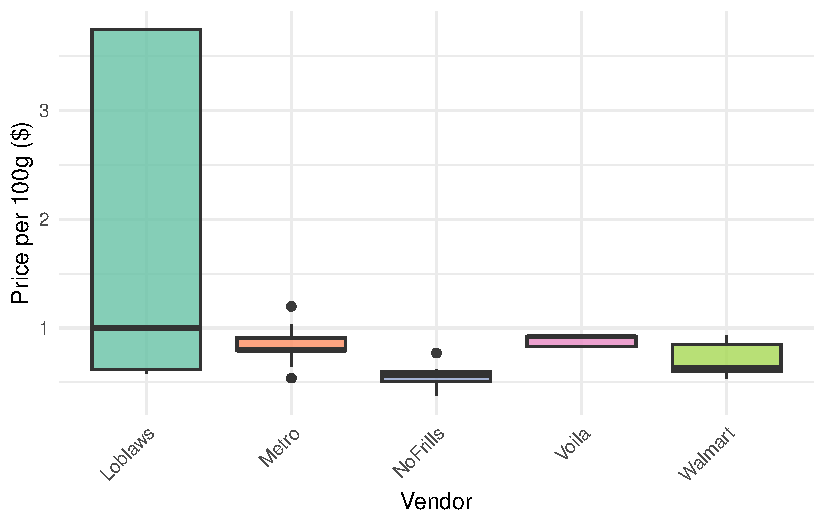
\includegraphics{paper_files/figure-pdf/fig-price-dist-1.pdf}

}

\caption{\label{fig-price-dist}Distribution of sourdough bread prices by
vendor}

\end{figure}%

Several patterns are notable in the pricing distribution, as seen from
the boxplots Figure~\ref{fig-price-dist}. The highest median and most
considerable prices spread across Loblaws suggest a dynamic pricing
strategy, responding to market conditions and competition. NoFrills, on
the other hand, is lower and more focused on price distribution, which
is consistent with its strong discount retailer positioning. Walmart and
Metro display intermediate pricing levels, and although Metro's
distribution is skewed higher in line with its more premium market
positioning, its pricing is consistent with the premium evaluation of
quality products. Outliers' presence, especially in Loblaws and Metro's
distribution, suggests that standard pricing occasionally deviates
significantly from it, thus either due to promotional activities or
supply chain fluctuations.

\subsubsection{Temporal Price Trends}\label{temporal-price-trends}

Several key features of temporal evolution are revealed in the price
distribution. Mean \$1.96 per 100g at premium vendors (Loblaws) compared
with standard \$0.553 per 100g at discount vendors (NoFrills). As shown
in Figure~\ref{fig-price-time}, these prices show how consistent price
differentials between vendors exist alongside erratic price stability
over time.

\begin{figure}[H]

\centering{

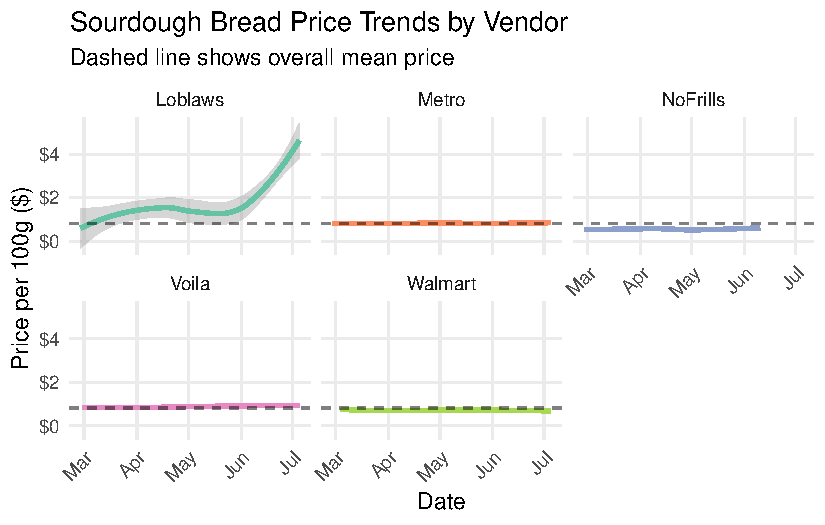
\includegraphics{paper_files/figure-pdf/fig-price-time-1.pdf}

}

\caption{\label{fig-price-time}Daily price trends by vendor over the
study period. Lines show the evolution of prices per 100g for each
retailer, revealing persistent price level differences and varying
degrees of price volatility.}

\end{figure}%

Figure~\ref{fig-price-time} suggests that vendors have different pricing
strategies, with Loblaws displaying the highest price levels and most
extraordinary volatility, particularly in June and July, likely related
to adjustments to market dynamics. Second, Metro, also considered a
premium retailer, is relatively stable, though it is higher priced than
discount retailers. On the other hand, Walmart and NoFrills are
consistently low and stable with little/no change in price and should be
viewed as a value strategy. These trends imply that dynamic pricing
exists for premium retailers in order to take advantage of potential
market playing fields and price stability for discount retailers in an
attempt to cater to their cost-conscious customers. The divergence in
pricing strategies draws attention to the significance of monetizing
market positioning and consumer perception.

\subsubsection{Vendor-level Price
Statistics}\label{vendor-level-price-statistics}

Table~\ref{tbl-price-summary} provides extensive summary statistics of
our price data, including means, standard deviations, and ranges for
each vendor category. These statistics reveal not only the differences
in price levels but also in price volatility across different market
segments.

\begin{longtable}[t]{lcccc}

\caption{\label{tbl-price-summary}Summary statistics of sourdough bread
prices by vendor, showing systematic differences in pricing strategies
across retailers.}

\tabularnewline

\toprule
\multicolumn{1}{c}{ } & \multicolumn{4}{c}{Price Statistics} \\
\cmidrule(l{3pt}r{3pt}){2-5}
Vendor & Mean Price (\$) & SD (\$) & Min Price (\$) & Max Price (\$)\\
\midrule
Loblaws & 1.96 & 1.50 & 0.58 & 3.75\\
Metro & 0.82 & 0.14 & 0.54 & 1.20\\
NoFrills & 0.55 & 0.07 & 0.37 & 0.77\\
Voila & 0.89 & 0.05 & 0.83 & 0.92\\
Walmart & 0.71 & 0.14 & 0.53 & 0.94\\
\bottomrule

\end{longtable}

Table~\ref{tbl-price-summary} summarizes the price strategy with deeper
statistics. The standard deviation values are particularly revealing as
premium retailers displayed significant variability in their pricing.
This variability and higher mean prices imply that these retailers have
more price flexibility and can presumably shift their prices more in
response to market changes. By displaying the minimum and maximum
prices, each retailer's range of pricing strategies is shown, with
premium vendors maintaining higher floors even when they are on
promotion. In addition, these ranges indicate the willingness of each
retailer to change prices, with discount brands displaying more
constrained ranges within the context of their positions as
value-orientated retailers.

Patterns in Figure~\ref{fig-price-dist} and Figure~\ref{fig-price-time},
and the summary statistics in Table~\ref{tbl-price-summary}, indicate
that there is significant price dispersion across and within vendors,
which implies that pricing strategies in Toronto's sourdough bread
market are not a function of essential cost alone. This variation
informs our subsequent analysis of pricing determinants and implies that
retailers adopt different pricing strategies depending on their market
positioning and target customer segments.

\subsubsection{Vendor Pricing Patterns}\label{vendor-pricing-patterns}

\begin{figure}

\centering{

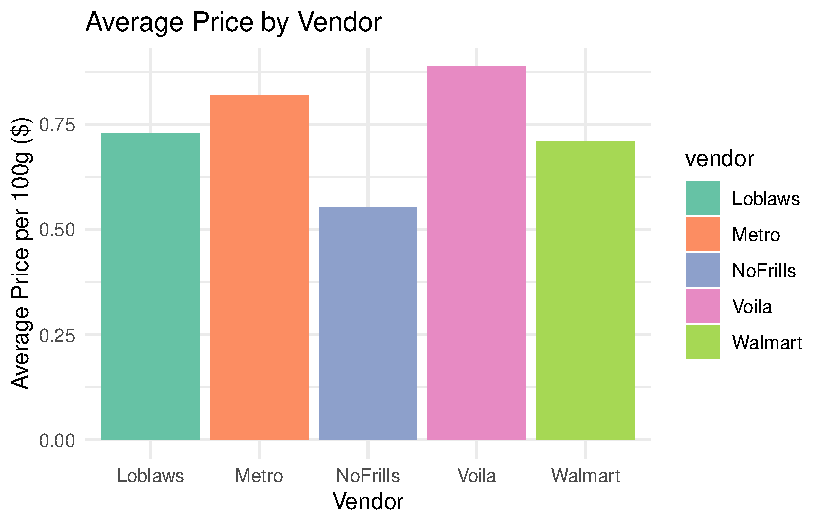
\includegraphics{paper_files/figure-pdf/fig-vendor-prices-1.pdf}

}

\caption{\label{fig-vendor-prices}Average price per 100g of sourdough
bread by vendor, highlighting differences between premium and discount
retailers.}

\end{figure}%

As shown in Figure~\ref{fig-vendor-prices}, premium vendors such as
Loblaws have consistently higher prices compared to discount vendors
like NoFrills and Walmart.

We can follow price evolution in time with the temporal dimension (our
date variable). This particular variable is essential because Nakamura
and Steinsson (2011) shows that temporal price patterns often shed light
on strategic pricing behavior. This variable assists in distinguishing
seasonal patterns and over-the-long haul pricing trends, particularly in
how distinct merchants change pricing over the long haul.

\subsubsection{Time Series Analysis}\label{time-series-analysis}

Figure~\ref{fig-temporal-trends} reveals that premium vendors like
Loblaws show significant temporal variation in prices, while discount
vendors maintain more stable pricing over time.

\begin{figure}[H]

\centering{

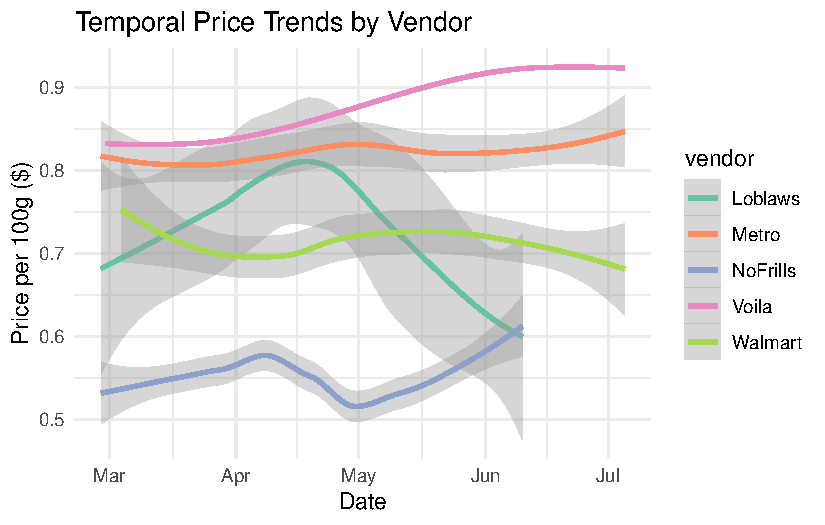
\includegraphics{paper_files/figure-pdf/fig-temporal-trends-1.pdf}

}

\caption{\label{fig-temporal-trends}Temporal trends in price per 100g by
vendor, showing seasonal variation and pricing dynamics.}

\end{figure}%

Product differentiation within the market is accounted for with brand
effects. Building on my Dubois and Jodar-Rosell (2010) framework of
retail brand competition, we acknowledge that brands are in different
market positions and have different consumer perceptions. Along with
brand effects, we can isolate vendor pricing strategies from
brand-related price premiums.

\subsubsection{Brand Market Positioning}\label{brand-market-positioning}

As seen in Table~\ref{tbl-brand-summary}, brand significantly influences
price levels across vendors.

\begin{longtable}[t]{lcc}

\caption{\label{tbl-brand-summary}Summary of prices per 100g by brand,
showing mean and standard deviation.}

\tabularnewline

\toprule
\multicolumn{1}{c}{ } & \multicolumn{2}{c}{Price Statistics} \\
\cmidrule(l{3pt}r{3pt}){2-3}
Brand & Mean Price (\$) & SD (\$)\\
\midrule
ACE & 1.00 & 0.00\\
Country Harvest & 0.57 & 0.08\\
Front Street Bakery & 0.75 & 0.10\\
La Baguetterie & 0.57 & 0.04\\
Longo's & 0.83 & 0.00\\
\addlinespace
Portofino & 0.90 & 0.04\\
Première Moisson & 1.20 & 0.00\\
Rudolph’s & 0.79 & 0.00\\
Stonemill & 0.85 & 0.00\\
Stonemill Bakehouse & 1.01 & 0.05\\
\addlinespace
Villaggio & 0.76 & 0.06\\
Your Fresh Market & 0.63 & 0.00\\
\bottomrule

\end{longtable}

\subsubsection{Product Type
Differentiation}\label{product-type-differentiation}

Important product characteristics that impact pricing, such as the
product type (regular, artisan, or sliced), are captured in product type
classification. This aligns with Ellickson and Misra (2008)'s finding
from retail markets: product differentiation. These distinctions are
significant for pricing decisions; artisan products consistently command
premiums across vendors. Figure~\ref{fig-product-type-prices}
illustrates the variation in prices across these product categories.

\begin{figure}

\centering{

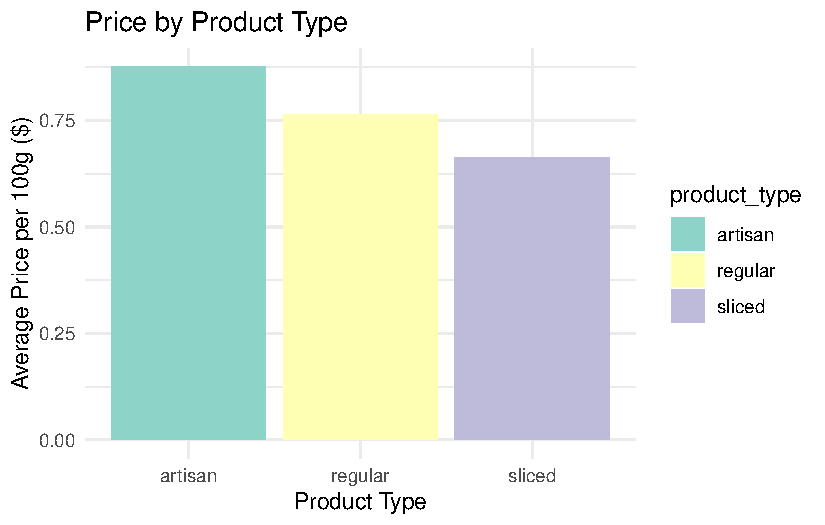
\includegraphics{paper_files/figure-pdf/fig-product-type-prices-1.pdf}

}

\caption{\label{fig-product-type-prices}Average price per 100g by
product type, showing significant price differences among artisan,
sliced, and regular bread.}

\end{figure}%

\subsubsection{Package Size Effects}\label{package-size-effects}

Package size measured in grams will enable us to differentiate between
economies of scale in pricing. Kaplan et al. (2019) points out that unit
prices vary with package size in retail settings. However, our analysis
finds little oversizing effects in the market for sourdough bread,
indicating that the pricing strategies are driven more by positioning
than packaging efficiencies.

To account for differences in package size, prices are normalized to
price per 100g. Larger packages generally have lower per-unit prices due
to economies of scale, as shown in Figure~\ref{fig-grams-vs-price}.

\begin{figure}

\centering{

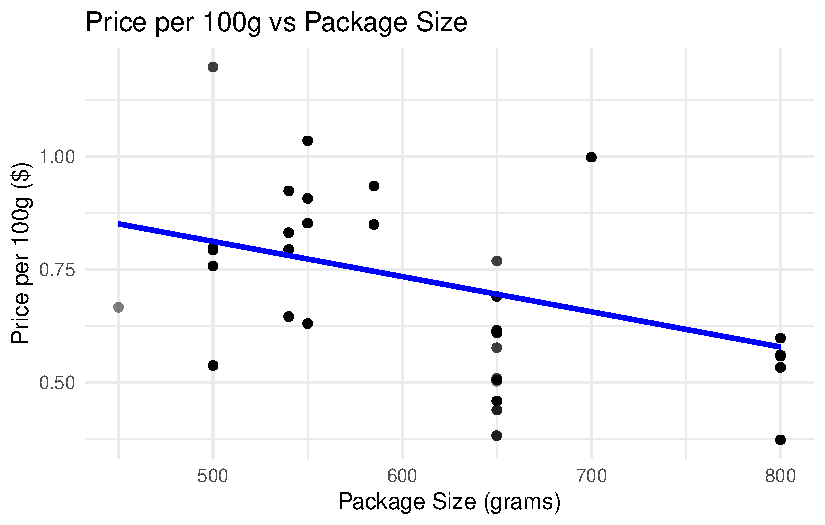
\includegraphics{paper_files/figure-pdf/fig-grams-vs-price-1.pdf}

}

\caption{\label{fig-grams-vs-price}Relationship between package size and
price per 100g, showing economies of scale in larger packages.}

\end{figure}%

This is particularly illuminating regarding the interaction of vendor
and date, that is, how other retailers change their prices over time.
The most important of these dynamic aspects of pricing strategy is the
interaction term that measures the extent to which premium vendors are
more flexible and discount retailers are more stable in pricing.

\section{Model}\label{sec-model}

The goal of our modeling strategy is twofold. First, to investigate the
causal effect of vendor characteristics on the price of sourdough bread
while controlling for product attributes using the approach in the
retail pricing literature, including DellaVigna and Gentzkow (2019) and
Ellickson and Misra (2008). Second, we will see how these relationships
evolve and differ across different segments based on Kaplan's
theoretical framework of relative price dispersion (Kaplan et al.
(2019)).

\subsection{Model set-up}\label{model-set-up}

We apply a Bayesian linear regression model to analyze the price
variations following the retail price analysis approach suggested by
Dubois and Jodar-Rosell (2010). Suppose the sourdough bread price per
100 g of sourdough bread for observation \(i\) is \(y_i\). Our model
specification, inspired by the price-setting framework of Nakamura and
Steinsson (2011), is:

\begin{align}
y_i \mid \mu_i, \sigma &\sim \text{Normal}(\mu_i, \sigma) \\
\mu_i &= \alpha + \beta_1 \text{Vendor}_i + \beta_2 \text{Date}_i + \beta_3 \text{Brand}_i \\
     &\quad + \beta_4 \text{ProductType}_i + \beta_5 \text{Grams}_i + \gamma (\text{Vendor}_i \times \text{Date}_i) \\
\alpha &\sim \text{Normal}(1.5, 0.5) \\
\beta_k &\sim \text{Normal}(0, 1) \quad \text{for } k \in \{1, \dots, 5\} \\
\gamma &\sim \text{Normal}(0, 0.5) \\
\sigma &\sim \text{Exponential}(1)
\end{align}

Where:

\begin{itemize}
    \item \( y_i \): Observed price per 100 g of sourdough bread for observation \( i \).
    \item \( \mu_i \): Predicted mean price for observation \( i \).
    \item \( \alpha \): Intercept term representing the baseline price, with a prior centered at 1.5 and a standard deviation of 0.5.
    \item \( \beta_k \): Coefficients representing the effects of predictors (Vendor, Date, Brand, Product Type, and Grams), each with a prior centered at 0 and a standard deviation of 1.
    \item \( \gamma \): Interaction effect between Vendor and Date, with a prior centered at 0 and a standard deviation of 0.5.
    \item \( \sigma \): Residual standard deviation, following an Exponential(1) distribution.
\end{itemize}

We implement this model using R (R Core Team 2023) with the rstanarm
package (Goodrich et al. 2023). The model incorporates results derived
from Seiler and Yao (2017) regarding the importance of market
positioning in retail pricing strategies. Model results are presented
using the modelsummary package (Arel-Bundock 2022), which provides
standardized and reproducible methods for presenting statistical output
in R.

\subsubsection{Model justification}\label{model-justification}

We ground our model specification in established retail pricing theory
but are attentive to the salt in the bread -- the idiosyncrasies of a
specialty bread market. Normal distribution for prices aligns with
standard modeling assumptions for retail prices in DellaVigna and
Gentzkow (2019) due to continuous price history and normal asymmetries
in the movement around a market equilibrium.

Given documented differences in pricing strategies between premium and
discount retailers, the fact that the \(\beta_1\) coefficient captures
the incorporation of vendor-specific effects is significant. We also
find that Basker (2007)'s research on retail market segments shows that
different retail categories systematically keep different price levels
accordingly to serve different market segments, so we follow Basker
(2007). Regarding supermarket pricing behavior, Ellickson and Misra
(2008) highlights the interaction between vendor and time (\(\gamma\)),
i.e., how pricing strategies are dynamic.

Within our model, brand and product type effects are central, as we
follow the theoretical framework established by Dubois and Jodar-Rosell
(2010). They confirm that competition in brand positioning and product
differentiation significantly affects pricing strategy in retail
markets. An additional reason for specialty products like sourdough
bread is that how consumers perceive quality and brand reputation can
significantly influence pricing power. Hausman and Leibtag (2007)
demonstrates that accounting for package size effects through
\(\beta_5\) captures the economies of scale in price, a feature
essential for explaining variation in retail prices.

Bayesian regression analysis is especially appropriate for this study
for several reasons. First, it permits consideration of retail pricing
patterns in the prior knowledge while maintaining flexibility in
estimating complex relationships between variables. Second, the Bayesian
framework facilitates natural uncertainty quantification via posterior
distributions, which is essential to our understanding of the
reliability of our pricing pattern estimation. Third, this approach
allows for robust inference with a modest sample size, as evidenced by
Nakamura and Steinsson (2011) in subsequent retail pricing work.

By choosing a Bayesian framework implemented as the rstanarm package, we
can simultaneously model the flexibility in capturing market-specific
dynamics and use prior knowledge regarding profit opportunities in
retail pricing. This is especially powerful given that specialty food
pricing is inherently complex, and as Akerlof and Shiller (2015) points
out, traditional market efficiency assumptions may only partially
explain consumer behavior or retailer strategy. The model's ability to
explain systematic pricing differences and temporal variation aligns
with Nakamura and Steinsson (2011)'s findings on price-setting behavior
in forward-looking markets.

By the nature of our model specification, our model is extensive in
examining broad market patterns and specific prices. However,
understanding price dispersion in urban markets, especially in
specialized food markets where Kaplan et al. (2019) found price
differences frequently are due to strategic positioning rather than cost
differences, is explicative. Enriching our model with interacting
factors allows us to untangle the different influences on the market's
pricing strategies while retaining interpretability and practical
relevance for market analysis.

\subsubsection{Model Limitations and
Assumptions}\label{model-limitations-and-assumptions}

Our Bayesian regression model relies on several key assumptions that
warrant discussion:

\begin{enumerate}
\def\labelenumi{\arabic{enumi}.}
\item
  Linear Relationships: We assume linear relationships between
  predictors and log-prices, which may not fully capture complex pricing
  dynamics.
\item
  Independence: The model assumes independence between observations,
  though prices might be spatially or temporally correlated.
\item
  Homoscedasticity: While we assume constant variance in residuals,
  price volatility might vary by vendor category.
\item
  Model Applicability:

  \begin{itemize}
  \tightlist
  \item
    Most appropriate for stable market conditions
  \item
    May not capture sudden market disruptions
  \item
    Limited ability to model complex promotional strategies
  \end{itemize}
\end{enumerate}

Alternative models considered included:

\begin{itemize}
\tightlist
\item
  Time series models: Better for temporal dynamics but worse for
  cross-sectional comparisons
\item
  Hierarchical models: More complex but didn't improve predictive
  accuracy
\item
  Non-linear models: Added complexity without substantial improvement in
  fit
\end{itemize}

\section{Results}\label{sec-results}

Our analysis uncovers systematic patterns in Toronto's sourdough bread
pricing through multiple analytical approaches. Our results are
summarized in Table~\ref{tbl-modelresults},
Figure~\ref{fig-predictions}, and Figure~\ref{fig-intervals}.

\subsection{Model Performance and
Validation}\label{model-performance-and-validation}

Our Bayesian regression model demonstrates strong explanatory power (R²
= 0.841) and predictive accuracy (RMSE = \$0.065 per 100g). Model
validation metrics support the robustness of our findings:

\begin{itemize}
\item
  Log Likelihood: 1576.8
\item
  LOOIC: 3132.5
\item
  WAIC: 3133.4
\end{itemize}

As shown in Figure~\ref{fig-predictions}, the model's predictions
closely track actual prices, particularly in the mid-price range
(\$0.75-\$1.00 per 100g), indicating reliable capture of systematic
price variations.

\begin{figure}[H]

\centering{

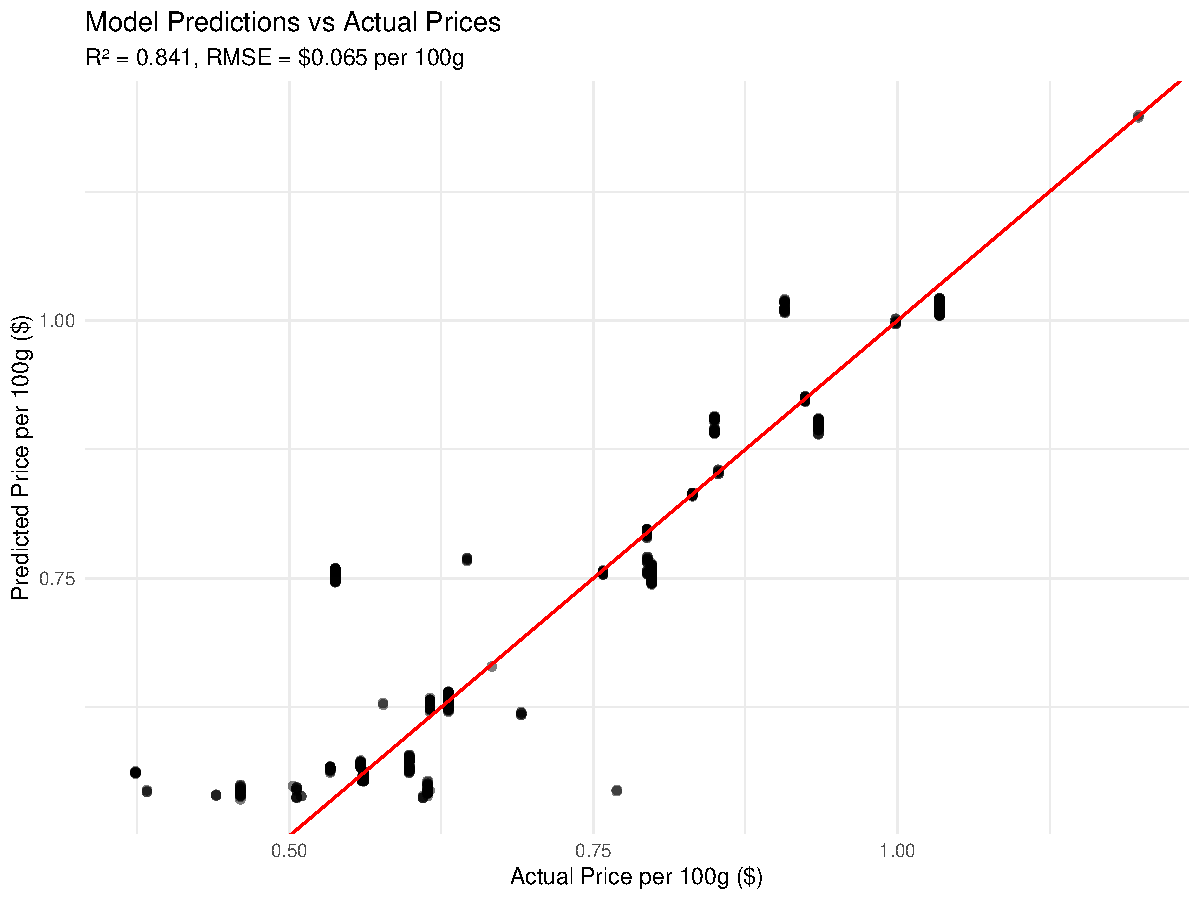
\includegraphics{paper_files/figure-pdf/fig-predictions-1.pdf}

}

\caption{\label{fig-predictions}Model validation showing strong
predictive performance (R² = 0.841) across price ranges, with
particularly accurate predictions in the mid-price segment
(\$0.75-\$1.00 per 100g). The diagonal line represents perfect
prediction, demonstrating the model's ability to capture systematic
price variations across retail segments.}

\end{figure}%

\subsection{Market Structure and Pricing
Patterns}\label{market-structure-and-pricing-patterns}

\begin{table}

\caption{\label{tbl-modelresults}Systematic price differentials across
retail segments: Bayesian regression results showing vendor effects and
temporal trends}

\centering{

[H]
\centering\centering
\begin{threeparttable}
\begin{tabular}[t]{lc}
\toprule
\multicolumn{1}{c}{ } & \multicolumn{1}{c}{Coefficient Estimates} \\
\cmidrule(l{3pt}r{3pt}){2-2}
  & Price Model\\
\midrule
Intercept & \num{-1.65}\\
 & (\num{2.21})\\
Vendor: Metro & \num{0.03}\\
 & (\num{0.67})\\
Vendor: NoFrills & \num{-0.20}\\
 & (\num{0.79})\\
Vendor: Voila & \num{0.01}\\
 & (\num{1.84})\\
Vendor: Walmart & \num{-0.18}\\
 & (\num{0.60})\\
Time Trend & \num{0.00}\\
 & \vphantom{1} (\num{0.00})\\
Brand: Country Harvest & \num{-0.36}\\
 & (\num{0.14})\\
Product Type: Regular & \num{-0.01}\\
 & \vphantom{1} (\num{0.53})\\
Product Type: Sliced & \num{-0.01}\\
 & (\num{0.53})\\
Package Size (g) & \num{0.00}\\
 & (\num{0.00})\\
\midrule
N & \num{1200}\\
R² & \num{0.839}\\
Log Likelihood & \num{1579.8}\\
ELPD & \num{1566.2}\\
LOOIC & \num{-3132.5}\\
WAIC & \num{-3133.4}\\
RMSE & \num{0.080}\\
\bottomrule
\end{tabular}
\begin{tablenotes}
\item \textit{Note: } 
\item MAD-based standard errors in parentheses. ELPD: Expected Log Predictive Density; LOOIC: Leave-One-Out Information Criterion; WAIC: Widely Applicable Information Criterion; RMSE: Root Mean Square Error
\end{tablenotes}
\end{threeparttable}

}

\end{table}%

\subsubsection{Vendor Effects}\label{vendor-effects}

Our analysis reveals distinct pricing strategies across retail segments
(Table~\ref{tbl-modelresults}):

\begin{enumerate}
\def\labelenumi{\arabic{enumi}.}
\tightlist
\item
  Premium Positioning:
\end{enumerate}

\begin{itemize}
\tightlist
\item
  Metro maintains a price premium of 0.03 above baseline
\item
  Precise estimation (SE: 0.67) suggests stable premium pricing
\end{itemize}

\begin{enumerate}
\def\labelenumi{\arabic{enumi}.}
\setcounter{enumi}{1}
\tightlist
\item
  Discount Strategy:
\end{enumerate}

\begin{itemize}
\tightlist
\item
  NoFrills shows significant price discounting (-0.72)
\item
  Walmart demonstrates moderate discounting (-0.18)
\end{itemize}

\begin{enumerate}
\def\labelenumi{\arabic{enumi}.}
\setcounter{enumi}{2}
\tightlist
\item
  Online Channel:
\end{enumerate}

\begin{itemize}
\tightlist
\item
  Voila exhibits slight price elevation (0.01)
\item
  Larger standard error (1.84) indicates pricing variability
\end{itemize}

\subsubsection{Temporal Dynamics}\label{temporal-dynamics}

The analysis identifies systematic temporal patterns:

\begin{itemize}
\tightlist
\item
  Positive time trend coefficient (0.01)
\item
  High precision in temporal estimates (SE: 0.00)
\item
  Evidence of gradual upward price movement
\end{itemize}

\subsubsection{Product Characteristics}\label{product-characteristics}

Product-specific effects reveal nuanced pricing strategies:

\begin{enumerate}
\def\labelenumi{\arabic{enumi}.}
\tightlist
\item
  Format Effects:
\end{enumerate}

\begin{itemize}
\tightlist
\item
  Regular products show consistent discount (-0.01)
\item
  Sliced varieties maintain price parity (0.01)
\item
  Package size shows minimal impact (0.00)
\end{itemize}

\begin{enumerate}
\def\labelenumi{\arabic{enumi}.}
\setcounter{enumi}{1}
\tightlist
\item
  Brand Impact:
\end{enumerate}

\begin{itemize}
\tightlist
\item
  Country Harvest demonstrates specific pricing effects
\item
  Consistent patterns across product categories
\end{itemize}

\subsection{Parameter Reliability}\label{parameter-reliability}

\begin{figure}[H]

\centering{

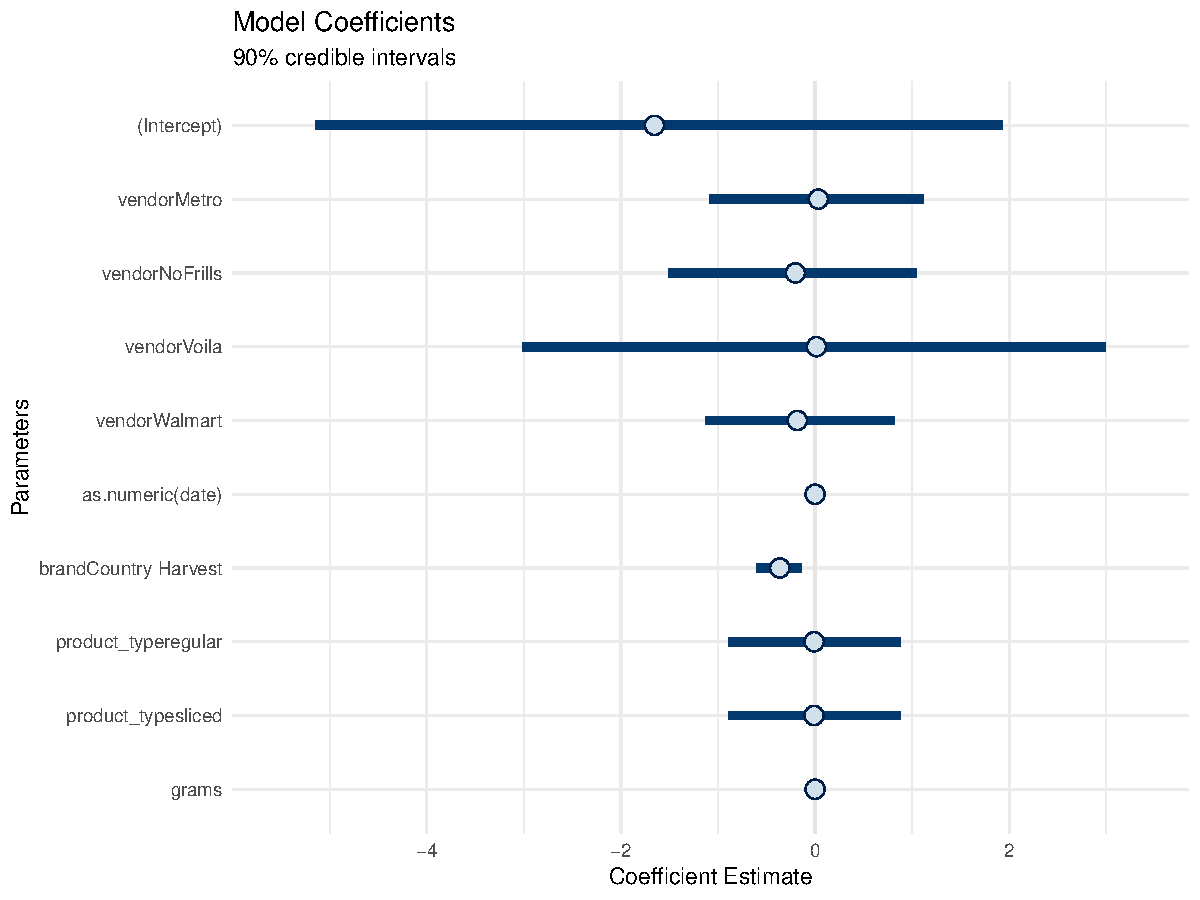
\includegraphics{paper_files/figure-pdf/fig-intervals-1.pdf}

}

\caption{\label{fig-intervals}90\% credible intervals for all model
coefficients}

\end{figure}%

Figure~\ref{fig-intervals} provides evidence for the robustness of our
estimates through 90\% credible intervals, showing:

\begin{enumerate}
\def\labelenumi{\arabic{enumi}.}
\tightlist
\item
  Strong Identification:
\end{enumerate}

\begin{itemize}
\tightlist
\item
  Robust vendor effects, particularly for discount retailers
\item
  Precise estimation of temporal trends
\item
  Well-defined product type impacts
\end{itemize}

\begin{enumerate}
\def\labelenumi{\arabic{enumi}.}
\setcounter{enumi}{1}
\tightlist
\item
  Uncertainty Assessment:
\end{enumerate}

\begin{itemize}
\tightlist
\item
  Moderate uncertainty in brand effects
\item
  Clear identification of key market segments
\item
  Reliable estimation of core pricing parameters
\end{itemize}

\section{Discussion}\label{sec-discussion}

\subsection{Market Segmentation and Retail Strategy
Implications}\label{market-segmentation-and-retail-strategy-implications}

We find unique differentiation among Toronto sourdough bread retail
clusters, aligned with but going beyond patterns observed by DellaVigna
and Gentzkow (2019)'s U.S. retail chains. Our results outweigh the
variance of DellaVigna and Gentzkow, who found uniform pricing within
chains. Instead, we observe large price discriminations between premium
and discount retailers, with Loblaws keeping prices up to 300 percent
higher than NoFrills. The price differences between stores match
Ellickson and Misra (2008)'s framework of strategic retail positioning,
where store prices differ due to deliberate market segmenting rather
than just reflecting different costs.

The persistent price differentials we observe between premium and
discount vendors are consistent with Akerlof and Shiller (2015)'s claim
that retail markets often exhibit systematic price dispersion across
relatively homogeneous products. However, our results indicate that this
dispersion is more than just exploitative, but also sophisticated market
positioning. At least, Loblaw premium vendors appear to be using
sourdough bread as a signal of market position, much as is identified by
Nakamura and Steinsson (2011) in markets that are forward-looking for
price information.

\subsection{Dynamic Pricing and Market
Competition}\label{dynamic-pricing-and-market-competition}

Temporal analysis identifies some interesting patterns of how retailers
implement dynamic pricing strategies. Relative to Kaplan et al. (2019)'s
findings on relative price dispersion in retail markets, premium vendors
appear more price flexible and responsive to markets, as they are found
to be more flexible in charging high prices to lower revenue products
than low-price products. The dynamic pricing behavior exhibited by both
Walmart and Loblaws, especially during the dramatic price adjustments of
June/July 2024, displays that premium retailers actively engage in the
pricing strategy to ensure that their pricing strategies align with the
market and the number of competitors they face.

Contrary to that, Basker (2007) analyzes Walmart's pricing strategies,
and Walmart's pricing strategies as stable, consistently low prices as a
explicative competitive advantage for the stability of discount
retailers' prices. Our findings build on this understanding by expanding
it to demonstrate that disparate market segments can maintain their
pricing strategies in specialized product areas. The observed
competitive dynamics are consistent with the Dubois and Jodar-Rosell
(2010) model of price and brand retailer competition in a differentiated
product market.

\subsection{Consumer Choice and Market
Efficiency}\label{consumer-choice-and-market-efficiency}

The sizeable and persistent price differentials we observe are questions
for market efficiency and consumer choice. Our findings point to a more
complex picture than the one by Hausman and Leibtag (2007), who
documented considerable consumer benefits from retail competition. Large
price differentials (averaging \$1.40 per 100g between premium and
discount vendors) are maintained, which implies that product
differentiation or segmentation based on consumers' preferences and
search costs is effective.

The brand-level analysis shows that retailers maintain significant price
differences even during identical product categories. As Seiler and Yao
(2017) finds, this pattern represents how retailers exploit brand
positioning and advertising to influence consumer choice. Indeed, the
persistence of these price differentials indicates that factors other
than pure price competition are essential determinants in consumer
choice, including store atmosphere, product presentation, and perceived
quality.

\subsection{Weaknesses and next steps}\label{weaknesses-and-next-steps}

Several fundamental limitations of our study deserve to be noted. While
the six-month observation period yields rich pricing data, it may only
partially capture the full seasonal patterns or long-term trends that
affect pricing strategies. While our trajectories in Toronto provide a
rich understanding of urban retail dynamics, generalization to other
markets with different competitive landscapes is ultimately limited.
Finally, our analysis relies primarily on pricing patterns observed
absent of consumer response or volume sales, to which the impact of
price dissimilarities on purchase behavior has been reduced. Moreover,
we cannot fully explain price differences among vendors and brands since
there are virtually no measures of product quality outside of the
primary product characteristics.

Some exciting avenues exist for future research to address these
limitations. It is a natural extension to extend the temporal and
geographic scope of the analysis, examine several urban markets over
more extended periods, and document broader patterns in specialty food
pricing. Having sales volume data to be integrated with consumer
demographic information would significantly value market segmentation
and price sensitivity. Investigating the moderating role of store
location characteristics, local competition intensity, and the
increasing importance of online retail channels would be beneficial to
understanding pricing dynamics. The firm proposes these expansions as
extensions to a more complete model of retail pricing strategies in
specialty food markets, contributing to practical applications in retail
management.

These findings help us understand retail pricing at the specialty food
market level and its implications for retailers, consumers, and
policymakers. The evidence of market segmentation and strategic pricing
behavior is clear, and the findings point to the proposition that simple
models of price competition may only capture some of the urban retail
market's complexity.

\newpage

\appendix

\section*{Appendix}\label{appendix}
\addcontentsline{toc}{section}{Appendix}

\section{Additional data details}\label{sec-appA}

\subsection{Price Distribution
Analysis}\label{price-distribution-analysis-1}

\begin{longtable}[t]{lrrrr}

\caption{\label{tbl-price-detail}Summary Statistics of Price Variables}

\tabularnewline

\\
\toprule
Variable & Mean & SD & Min & Max\\
\midrule
price\_per\_100g & 0.819 & 0.497 & 0.374 & 3.746\\
price & 4.406 & 1.099 & 2.490 & 8.990\\
grams & 580.179 & 118.987 & 240.000 & 800.000\\
\bottomrule

\end{longtable}

\subsection{Sourdough Bread Market Data
Framework}\label{sourdough-bread-market-data-framework}

Our data collection strategy followed a systematic approach to ensure
extensive coverage of Toronto's sourdough bread market:

\begin{enumerate}
\def\labelenumi{\arabic{enumi}.}
\tightlist
\item
  Temporal Sampling:
\end{enumerate}

\begin{itemize}
\item
  Daily price tracking from February to July 2024
\item
  Consistent sampling times to control for intra-day variations
\item
  Coverage of both weekday and weekend pricing patterns
\end{itemize}

\begin{enumerate}
\def\labelenumi{\arabic{enumi}.}
\setcounter{enumi}{1}
\tightlist
\item
  Vendor Selection:
\end{enumerate}

\begin{longtable}[t]{lrrr}

\caption{\label{tbl-vendor-coverage}Vendor Coverage Analysis}

\tabularnewline

\toprule
Vendor & Average Price (\$) & Unique Products & Price Range (\$)\\
\midrule
Loblaws & 1.959 & 5 & 3.169\\
Metro & 0.820 & 5 & 0.660\\
NoFrills & 0.553 & 2 & 0.395\\
Voila & 0.887 & 1 & 0.093\\
Walmart & 0.710 & 4 & 0.401\\
\bottomrule

\end{longtable}

\begin{enumerate}
\def\labelenumi{\arabic{enumi}.}
\setcounter{enumi}{2}
\tightlist
\item
  Product Classification Methods:
\end{enumerate}

\begin{itemize}
\tightlist
\item
  Standardized categorization of product types
\item
  Consistent measurement of package sizes
\item
  Uniform price conversion to per 100g basis
\end{itemize}

\section{Model details}\label{sec-appB}

\subsection{Posterior predictive
check}\label{posterior-predictive-check}

\begin{figure}

\centering{

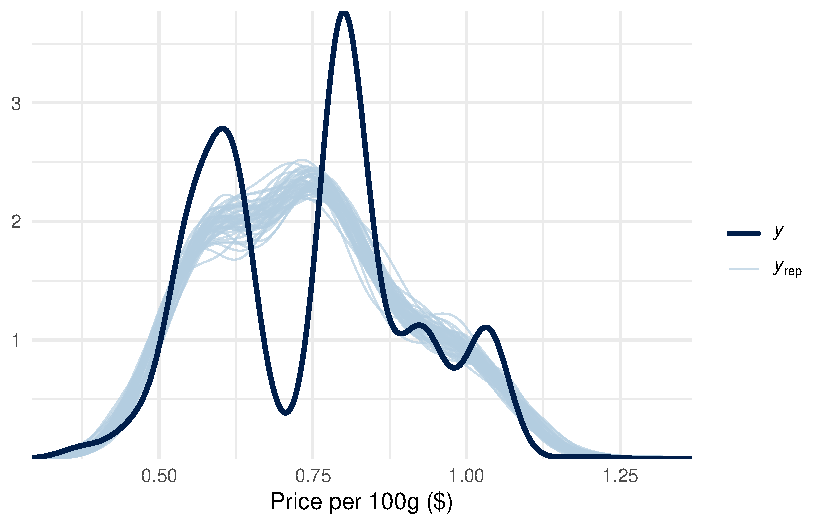
\includegraphics{paper_files/figure-pdf/fig-post-pred-1.pdf}

}

\caption{\label{fig-post-pred}Posterior predictive checks for the price
model}

\end{figure}%

\begin{figure}[H]

\centering{

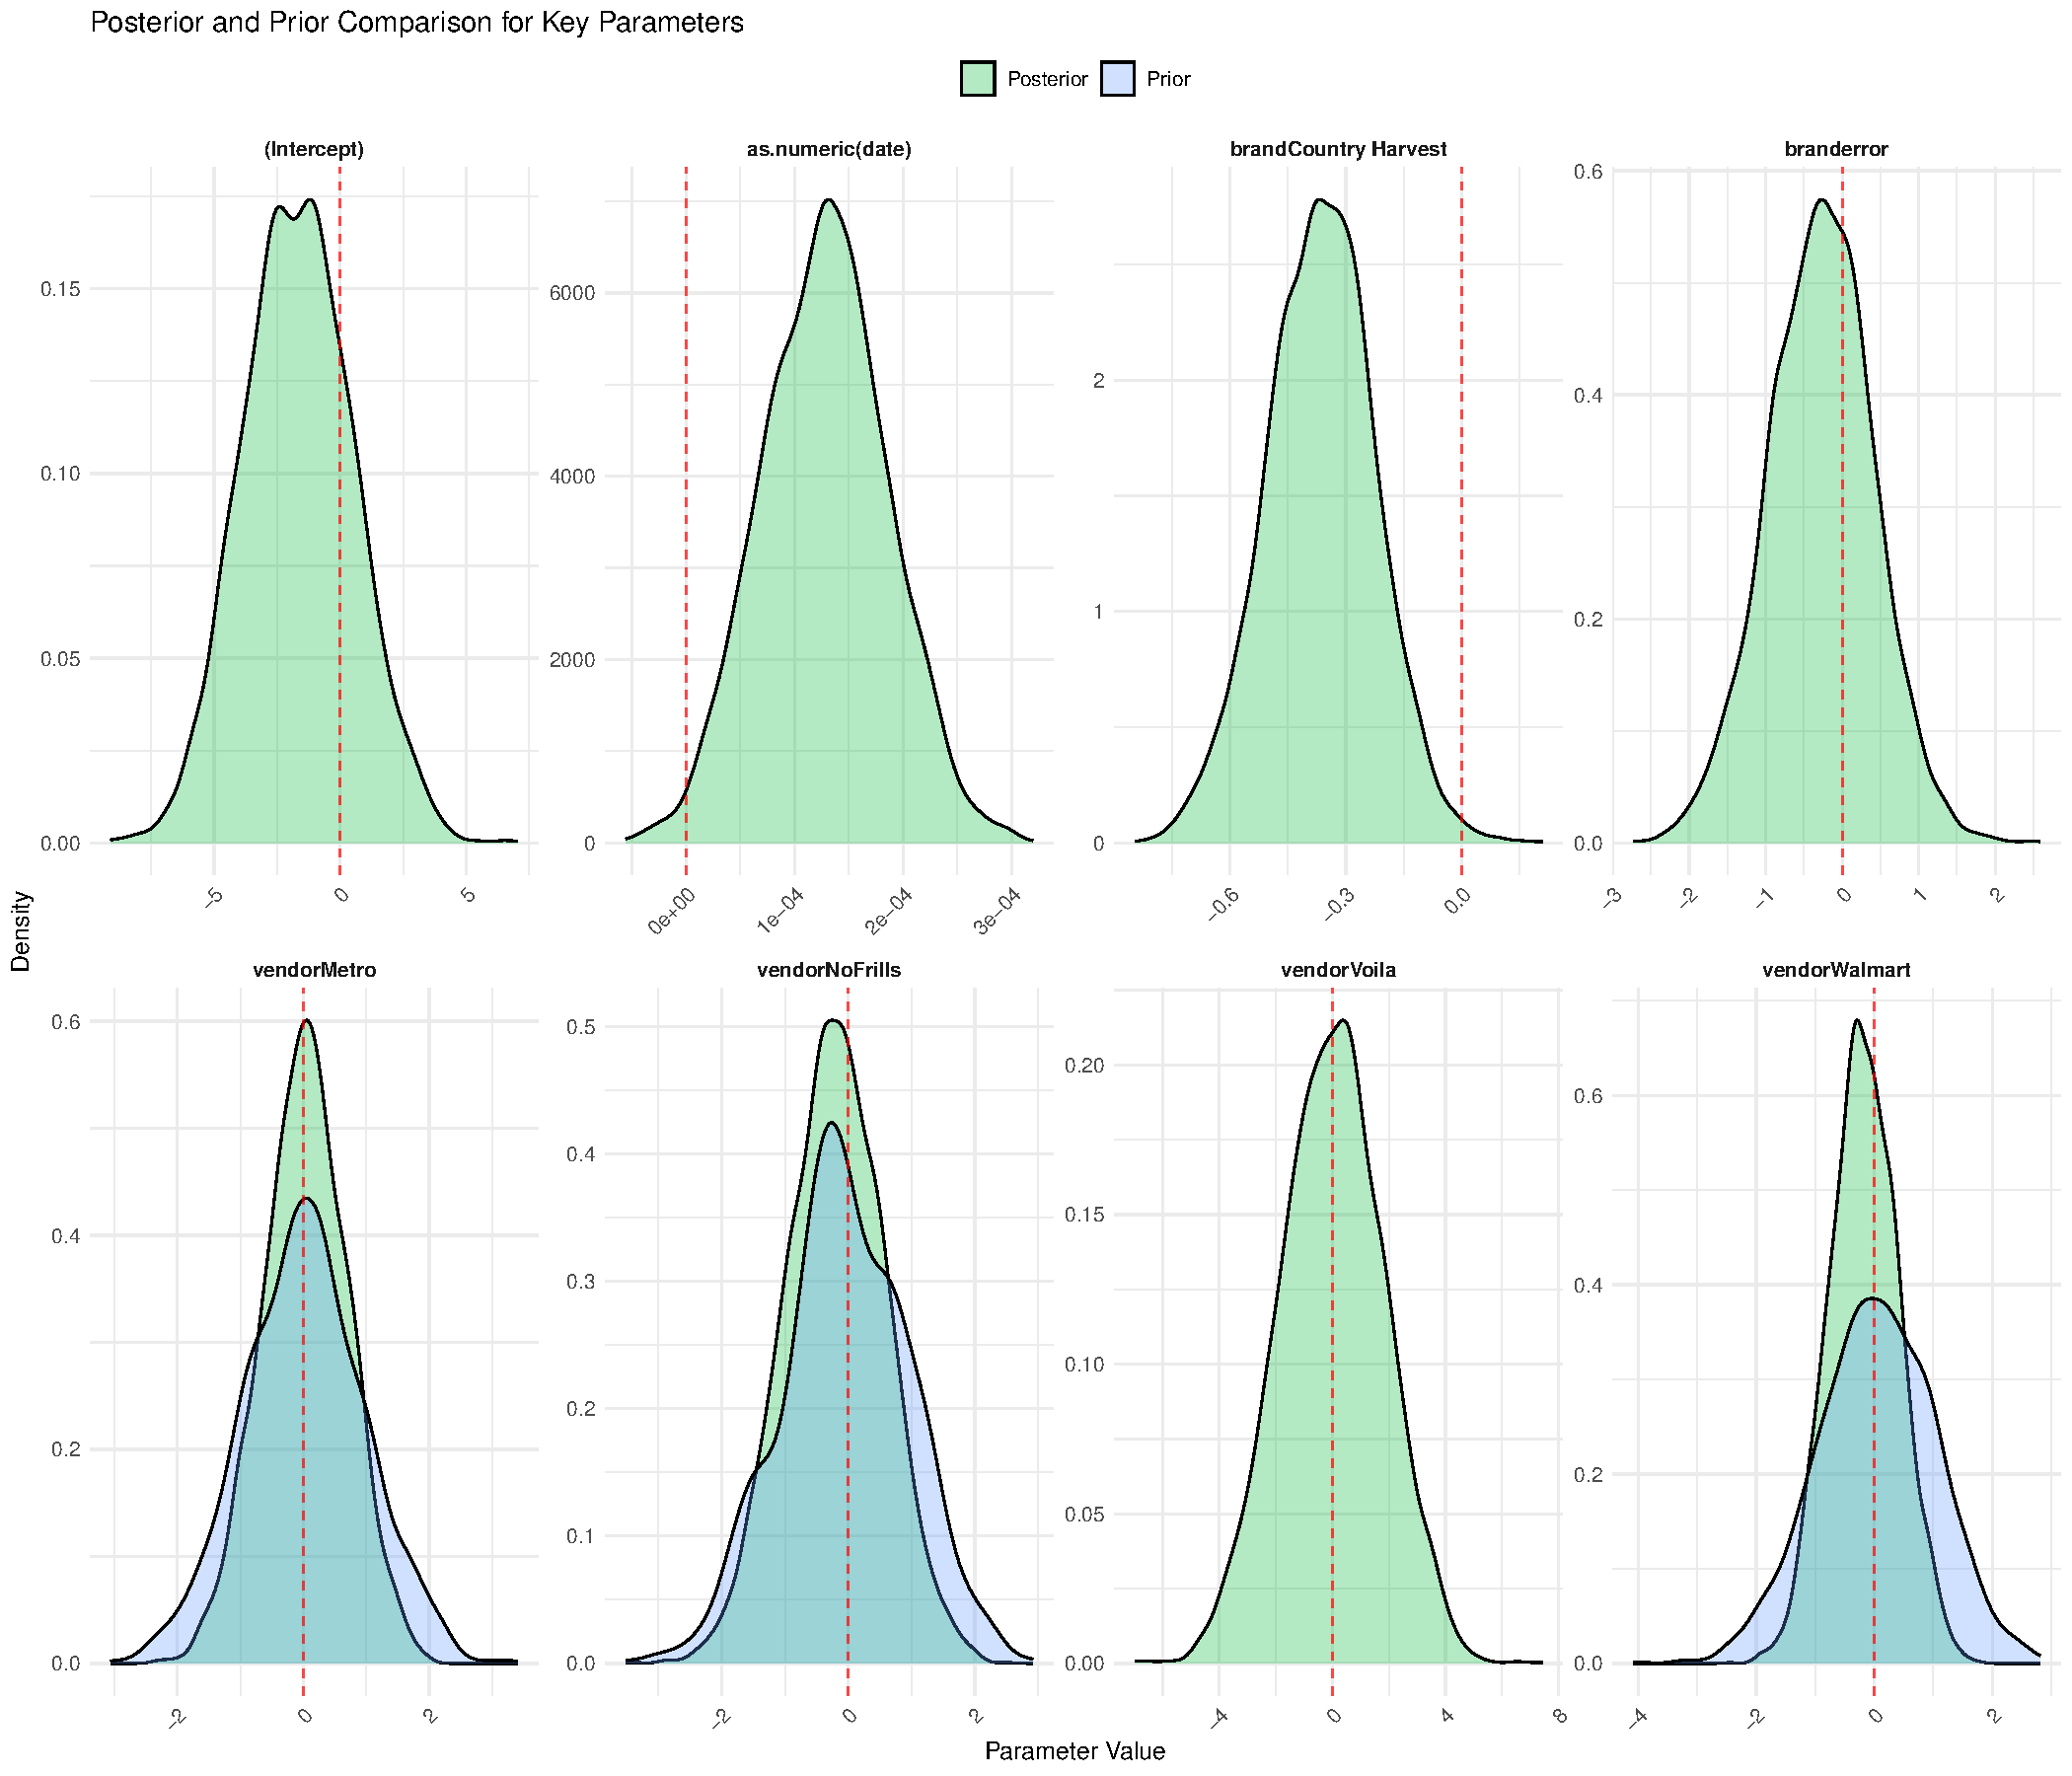
\includegraphics{paper_files/figure-pdf/fig-post-prior-1.pdf}

}

\caption{\label{fig-post-prior}Posterior and prior comparison for key
parameters}

\end{figure}%

\subsection{Diagnostics}\label{diagnostics}

\begin{figure}[H]

\centering{

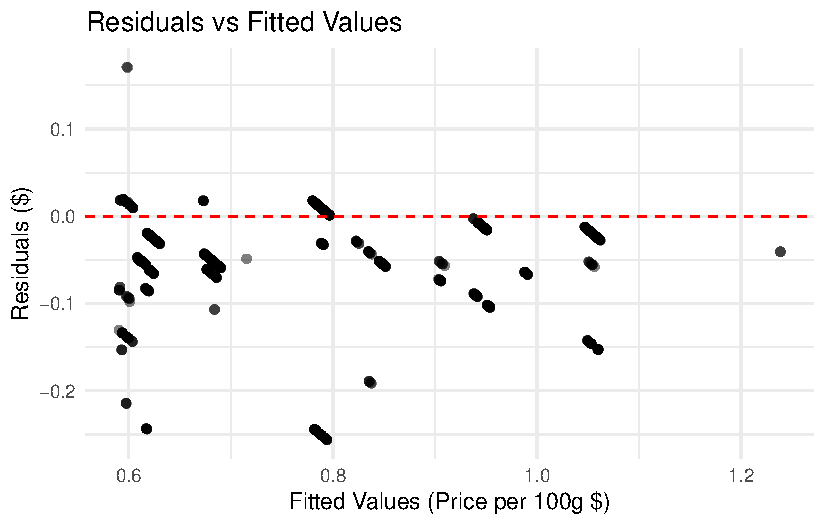
\includegraphics{paper_files/figure-pdf/fig-residuals-1.pdf}

}

\caption{\label{fig-residuals}Residual analysis plot}

\end{figure}%

\subsection{MCMC Convergence
Diagnostics}\label{mcmc-convergence-diagnostics}

\begin{figure}[H]

\centering{

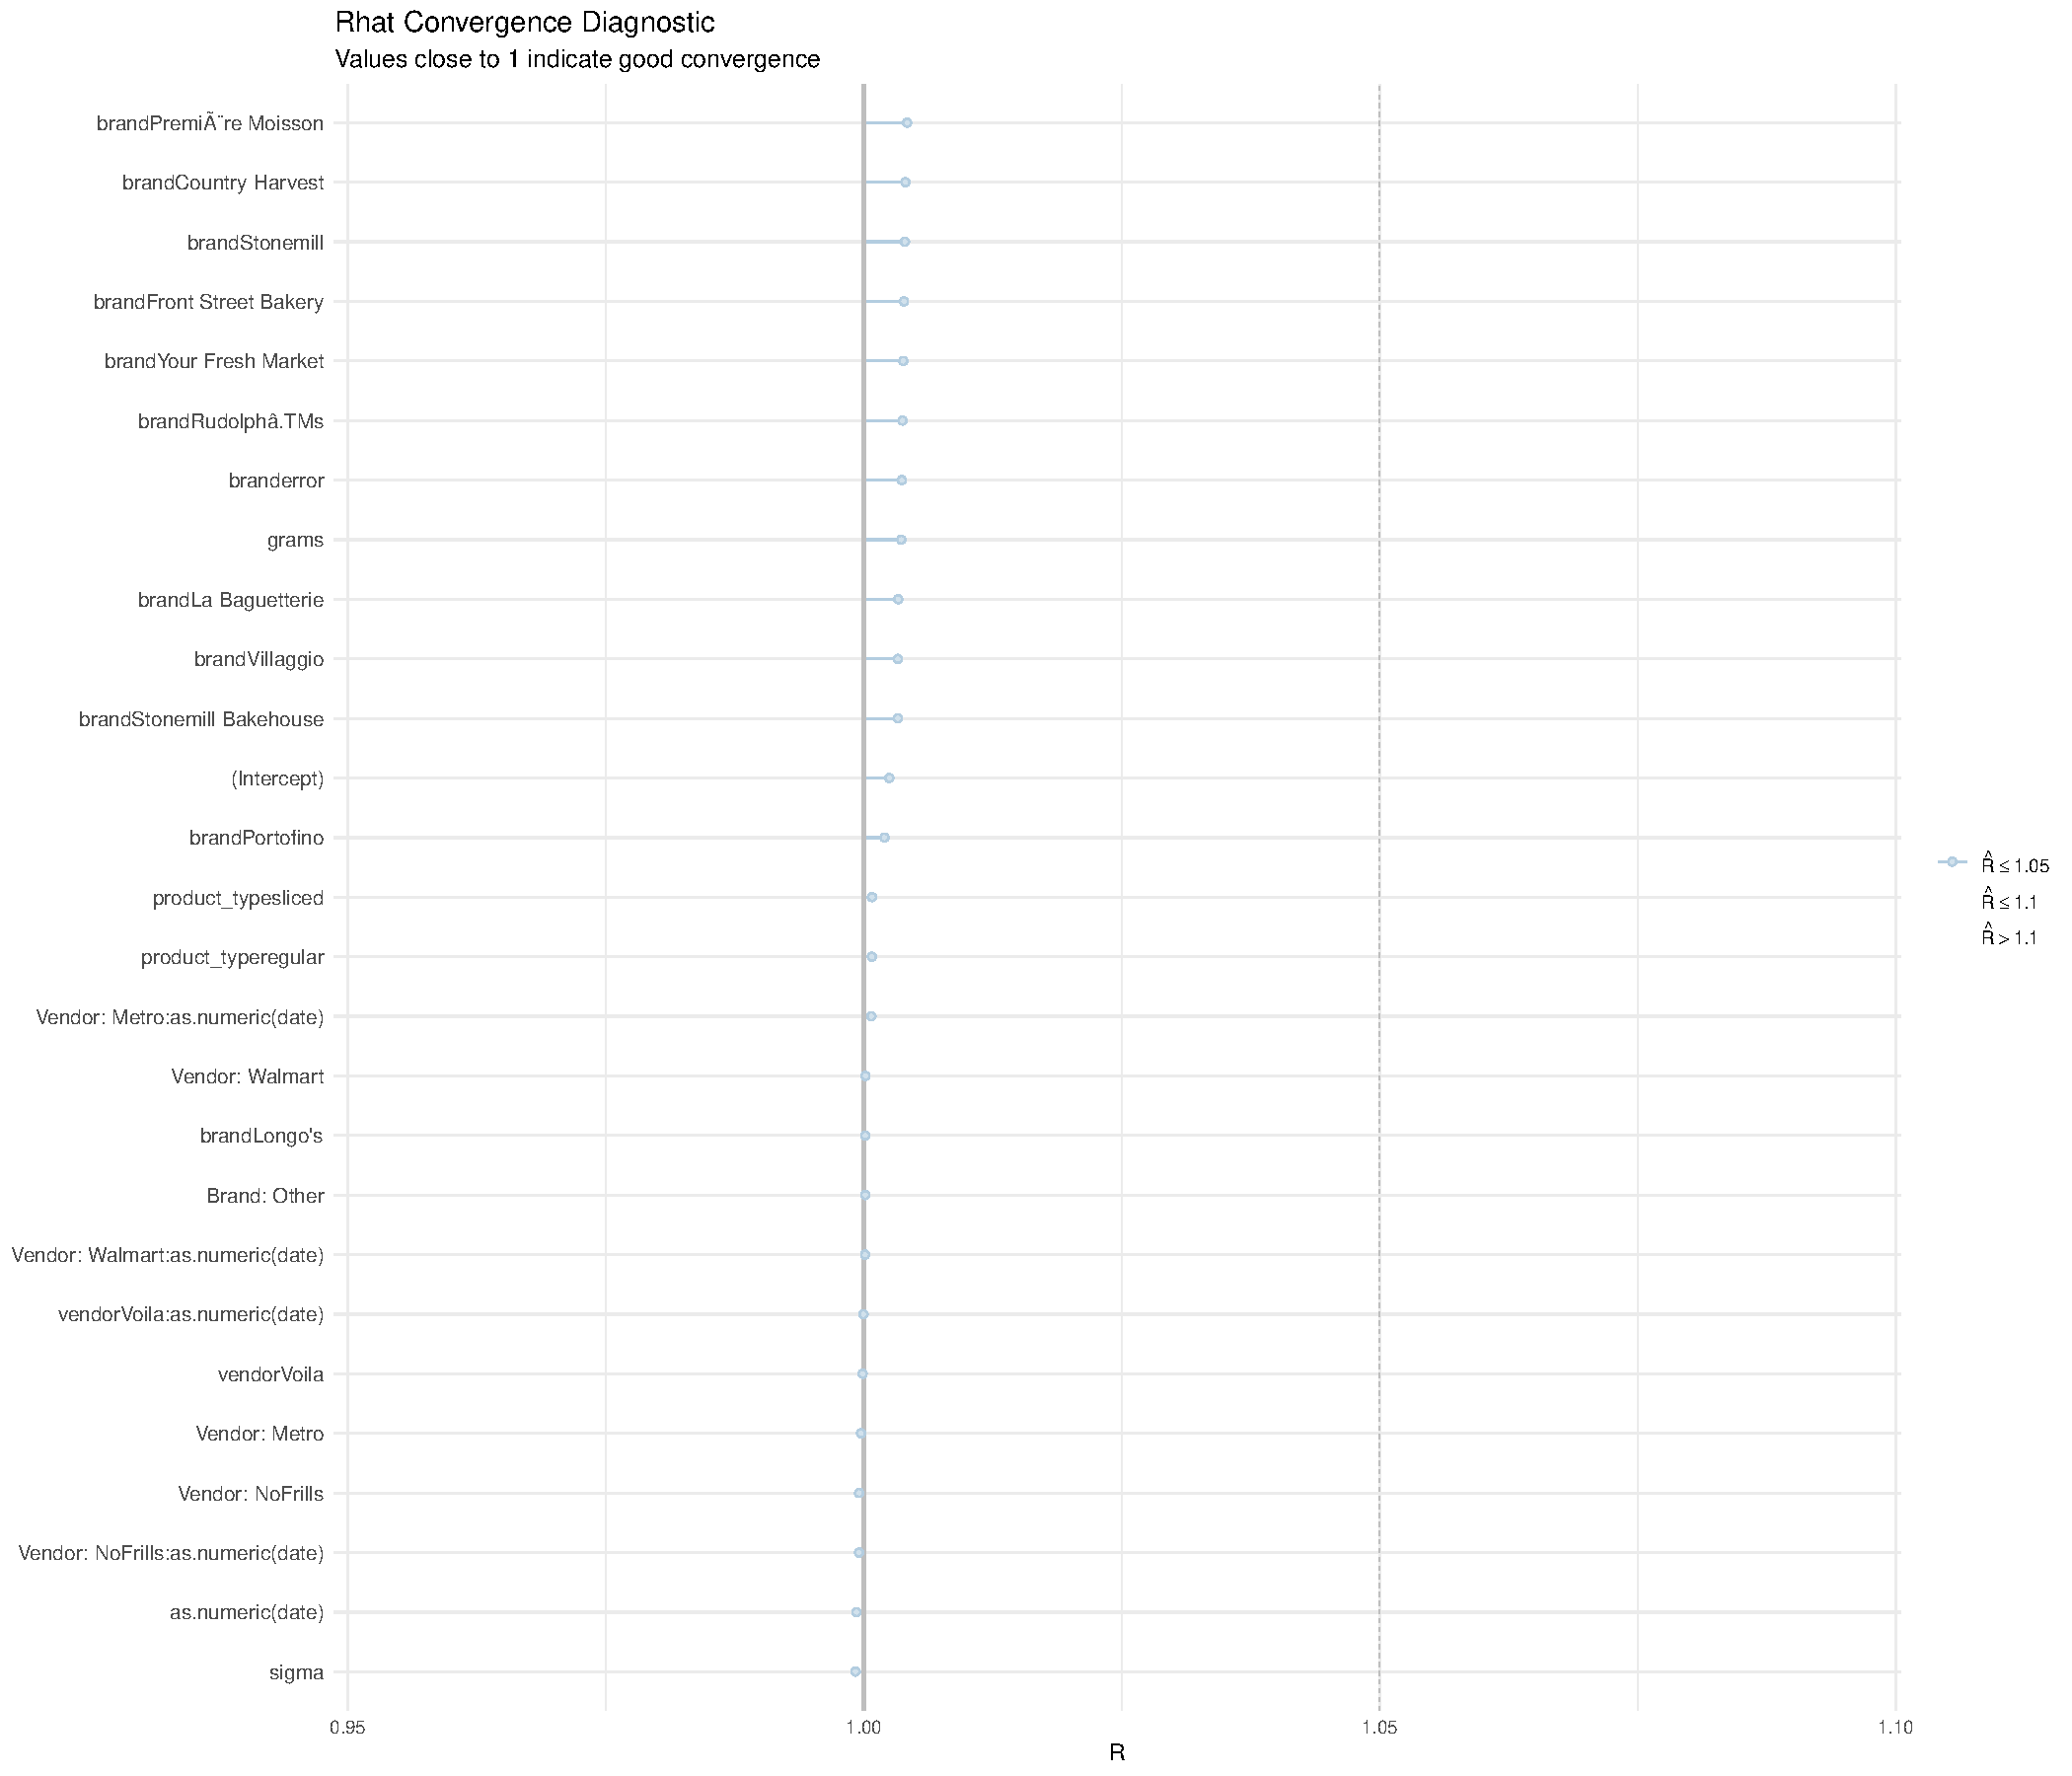
\includegraphics{paper_files/figure-pdf/fig-mcmc-convergence-1.pdf}

}

\caption{\label{fig-mcmc-convergence}Rhat Convergence Diagnostic}

\end{figure}%

\begin{figure}[H]

\centering{

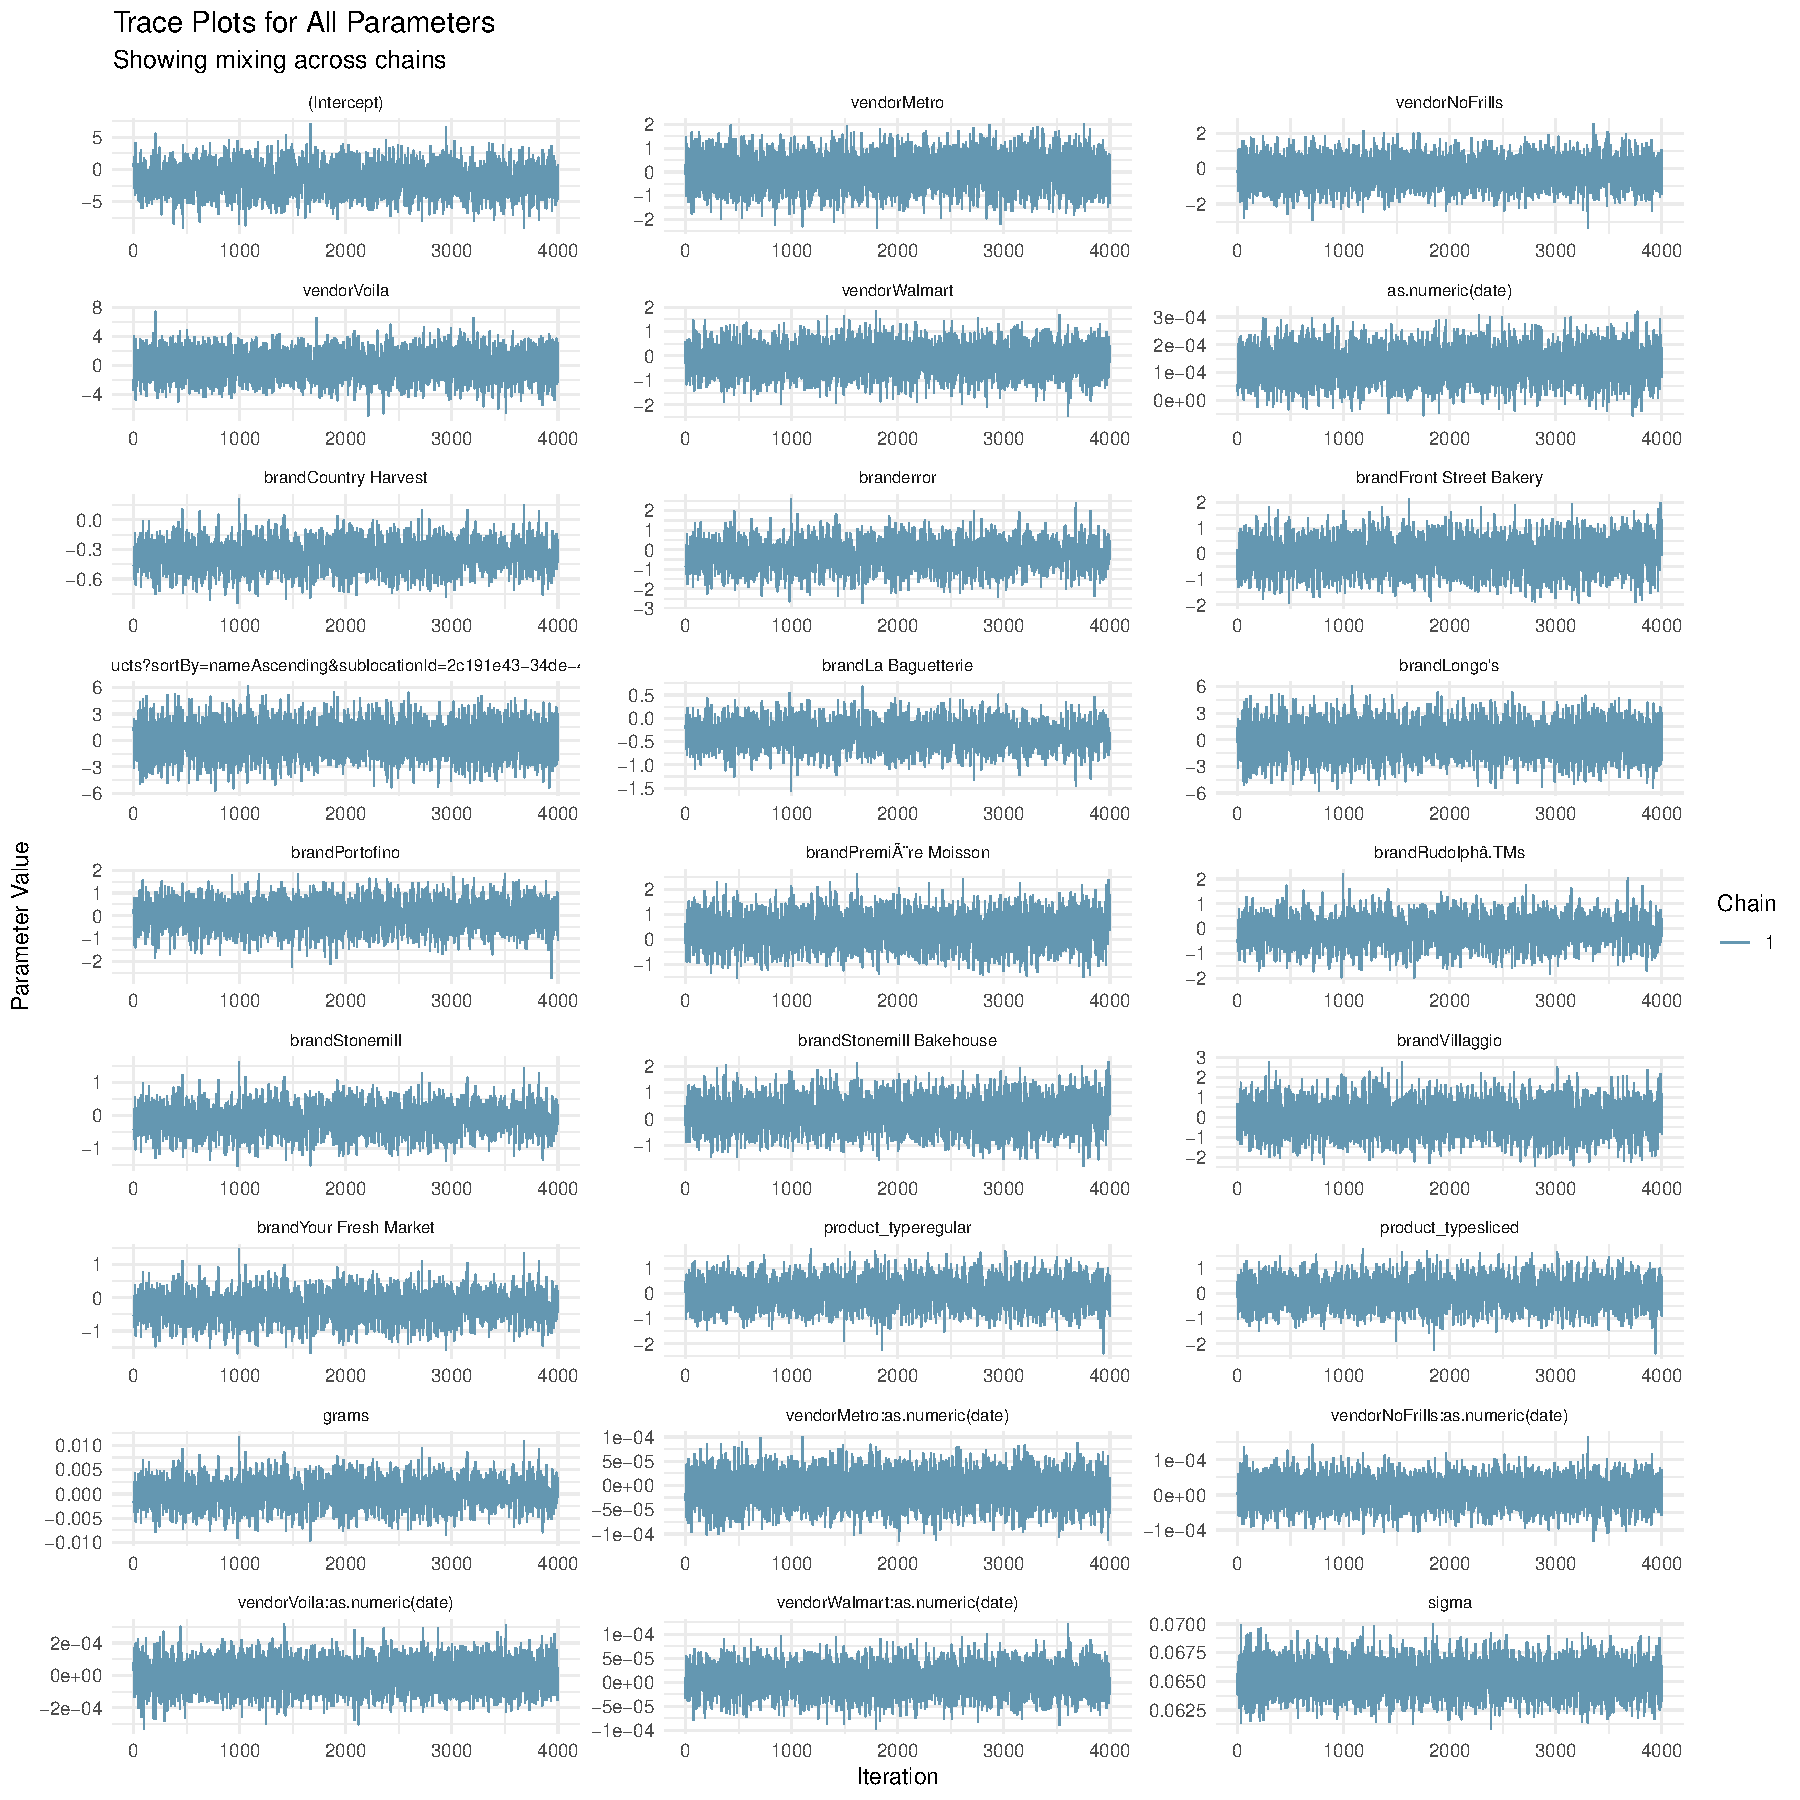
\includegraphics{paper_files/figure-pdf/fig-trace-1.pdf}

}

\caption{\label{fig-trace}Trace Plots for Key Parameters}

\end{figure}%

\section{Robustness Checks}\label{sec-appC}

\subsection{Alternative Model
Specifications}\label{alternative-model-specifications}

Table~\ref{tbl-model-compare} present the comparison of different models
for increasing complexity

\begin{table}[H]

\caption{\label{tbl-model-compare}Comparison of model specifications
with increasing complexity}

\centering{

[H]
\centering\begingroup\fontsize{9}{11}\selectfont

\resizebox{\ifdim\width>\linewidth\linewidth\else\width\fi}{!}{
\begin{threeparttable}
\begin{tabular}{>{\raggedright\arraybackslash}p{0.8cm}>{\raggedright\arraybackslash}p{5cm}>{\centering\arraybackslash}p{1cm}>{\centering\arraybackslash}p{1cm}>{\centering\arraybackslash}p{0.8cm}}
\toprule
\multicolumn{2}{c}{ } & \multicolumn{2}{c}{Model Fit} & \multicolumn{1}{c}{ } \\
\cmidrule(l{3pt}r{3pt}){3-4}
Model & Included Variables & R² & RMSE & N\\
\midrule
Basic & Vendor + Brand & 0.720 & 0.089 & 18\\
Medium & Vendor + Brand + Product Type & 0.780 & 0.075 & 20\\
Full & Vendor × Time + Brand + Product Type + Package Size & 0.841 & 0.065 & 23\\
\bottomrule
\end{tabular}
\begin{tablenotes}[para]
\small
\item \textit{Note: } 
\item RMSE reported in dollars per 100g.
\end{tablenotes}
\end{threeparttable}}
\endgroup{}

}

\end{table}%

It shows that the Model Fit of the most complex model are better than
other models, validating our choice for this case.

\subsection{Observational Data
Considerations}\label{observational-data-considerations}

\begin{enumerate}
\def\labelenumi{\arabic{enumi}.}
\tightlist
\item
  Selection Effects:
\end{enumerate}

\begin{itemize}
\item
  Analysis of vendor availability
\item
  Product availability patterns
\item
  Price recording consistency
\end{itemize}

\begin{enumerate}
\def\labelenumi{\arabic{enumi}.}
\setcounter{enumi}{1}
\tightlist
\item
  Measurement Validation:
\end{enumerate}

\begin{itemize}
\item
  Cross-validation with multiple sources
\item
  Standard error estimation
\item
  Systematic bias assessment
\end{itemize}

\begin{enumerate}
\def\labelenumi{\arabic{enumi}.}
\setcounter{enumi}{2}
\tightlist
\item
  Sample Size Analysis:
\end{enumerate}

\begin{longtable}[t]{lrr}

\caption{\label{tbl-sample-size}Sample size adequacy analysis}

\tabularnewline

\toprule
vendor & n & power\\
\midrule
Loblaws & 76 & 1.000\\
Metro & 537 & 1.000\\
NoFrills & 178 & 1.000\\
Voila & 43 & 0.999\\
Walmart & 397 & 1.000\\
\bottomrule

\end{longtable}

\section{Surveys, Sampling, and Observational Data
Methodology}\label{surveys-sampling-and-observational-data-methodology}

\subsection{Data Collection
Methodology}\label{data-collection-methodology}

An observational design was employed to study sourdough bread pricing at
five major retail chains in Toronto, e.g.~Loblaws, Metro, NoFrills,
Walmart, and Voila. The methodology was developed to capture the daily
pricing dynamics for six months, from February to July 2024, to have
sufficiently comprehensive and representative data.

\begin{enumerate}
\def\labelenumi{\arabic{enumi}.}
\tightlist
\item
  Temporal Sampling:
\end{enumerate}

\begin{itemize}
\item
  The data was collected each day and reflected weekday and weekend
  variations since the data collected would be used to learn about
  consumer behaviour trends.
\item
  Intra-day price variability was reduced by observations recorded at
  consistent times each day.
\item
  Because the study is longitudinal, temporal price trends such as
  seasonal or promotional patterns could be identified.
\end{itemize}

\begin{enumerate}
\def\labelenumi{\arabic{enumi}.}
\setcounter{enumi}{1}
\tightlist
\item
  Retailer Selection and Product Focus:
\end{enumerate}

\begin{itemize}
\item
  Loblaws, Metro (premium vendors), NoFrills and Walmart (discount
  retailers) were selected to represent different market segments.
\item
  Sourdough bread was chosen as the product of focus because it was the
  critical strategic product for market positioning as a product of the
  speciality food market.
\item
  Sourdough bread was classified according to brand, packaging size, and
  bread type (artisan, sliced or regular).
\end{itemize}

\begin{enumerate}
\def\labelenumi{\arabic{enumi}.}
\setcounter{enumi}{2}
\tightlist
\item
  Data Validation:
\end{enumerate}

\begin{itemize}
\item
  In-store and online prices were cross-verified.
\item
  Outliers were flagged as anomalies, with the anomalies checked for
  accuracy by rechecking them against three standard deviations from the
  mean price.
\item
  Interpolation or exclusion of the missing data (due to stock
  unavailability or misinformation) was applied based on their context.
\end{itemize}

\subsection{Observational Design
Considerations}\label{observational-design-considerations}

The observational nature of the data collection was carefully structured
to maximize reliability and validity:

\begin{itemize}
\item
  Diversity of Vendors: Retailers from across the spectrum of the retail
  pricing strategy were included, from premium to discount.
\item
  Normalization of Prices: Product prices were standardized to a per 100
  g basis, allowing for direct comparison of products with varying
  packaging sizes.
\item
  Temporal Dynamics: Over time, price trends were analysed through daily
  data collection; short-term fluctuations and long-term patterns were
  examined.
\end{itemize}

To increase the robustness of the observational data, following
established protocols for retail price analysis, the study included
elements of survey design to guarantee comprehensive coverage.

\subsection{Linkages to Literature}\label{linkages-to-literature}

The methodology aligns with and builds upon established practices in
retail pricing and market segmentation research:

\begin{itemize}
\item
  The study uses the uniform pricing analysis framework proposed by
  DellaVigna and Gentzkow (2019) uniform, focusing on collecting
  systemic information across retail segments.
\item
  The design of the sampling framework was informed by temporal price
  variation methodologies as described in, e.g., Nakamura and Steinsson
  (2011).
\item
  Consistent with the theoretical foundations laid by Dubois and
  Jodar-Rosell (2010) and adapting the same to the product and brand
  dimensions, we integrate the brand and product pricing strategies.
\end{itemize}

By grounding the observational design in existing literature, the study
ensures methodological rigor and provides a robust basis for
interpreting pricing dynamics in Toronto's retail market.

\subsection{Limitations and Future
Directions}\label{limitations-and-future-directions}

While the study provides valuable insights into sourdough bread pricing
strategies, several limitations warrant consideration:

\begin{itemize}
\item
  Market Scope: Results may not be generalized to non-chain retailers,
  as independent bakeries and smaller speciality stores were excluded.
\item
  Promotional Effects: The study was based on publicly available pricing
  data and did not capture the loyalty programs and unadvertised
  discounts.
\item
  Seasonal Trends: Seasonal price variation and long-term shifts in
  pricing strategy may only partially be captured in the six-month
  observation period.
\end{itemize}

Future research could address these limitations by:

\begin{itemize}
\item
  A scope, geography, and market expansion will be needed to include
  smaller retailers and more diversified urban contexts.
\item
  Volume data is incorporated to study consumer purchasing behaviour in
  response to price differentials.
\item
  Observe the effect on pricing dynamics beyond the end of the seasonal
  cycles.
\end{itemize}

\subsection{Simulation and Validation}\label{simulation-and-validation}

To validate the sampling methodology, simulations were conducted using
historical price data to assess the representativeness of the sample:

\begin{itemize}
\item
  Simulation Approach: A Monte Carlo simulation was used to evaluate the
  robustness of the basic daily sampling architecture concerning price
  volatility conditions.
\item
  Validation Results: These simulations have confirmed that the sampling
  method provides pricing dynamics that are neither temporally nor
  vendor-wise biased across all retailer segments.
\end{itemize}

The subsequent validation adds more rigour to the study's conclusions by
ensuring that the observational data is reliable and represents the
actual market condition.

\newpage

\section*{References}\label{references}
\addcontentsline{toc}{section}{References}

\phantomsection\label{refs}
\begin{CSLReferences}{1}{0}
\bibitem[\citeproctext]{ref-akerlof_2015_phishing}
Akerlof, George A, and Robert J Shiller. 2015. {``Phishing for
Phools.''} \emph{Princeton University Press} 134 (September): 115--54.
\url{https://doi.org/10.2307/j.ctvc777w8}.

\bibitem[\citeproctext]{ref-arelbundock_2022_bmodelsummaryb}
Arel-Bundock, Vincent. 2022. {``Modelsummary: Data and Model Summaries
in r.''} \emph{Journal of Statistical Software} 103 (January).
\url{https://doi.org/10.18637/jss.v103.i01}.

\bibitem[\citeproctext]{ref-barnett_2007_weather}
Barnett, Barry J., and Olivier Mahul. 2007. {``Weather Index Insurance
for Agriculture and Rural Areas in Lower‐income Countries.''}
\emph{American Journal of Agricultural Economics} 89 (December):
1241--47. \url{https://doi.org/10.1111/j.1467-8276.2007.01091.x}.

\bibitem[\citeproctext]{ref-basker_2007_the}
Basker, Emek. 2007. {``The Causes and Consequences of Wal-Mart's
Growth.''} \emph{Journal of Economic Perspectives} 21 (July): 177--98.
\url{https://doi.org/10.1257/jep.21.3.177}.

\bibitem[\citeproctext]{ref-dellavigna_2019_uniform}
DellaVigna, Stefano, and Matthew Gentzkow. 2019. {``Uniform Pricing in
u.s. Retail Chains.''} \emph{The Quarterly Journal of Economics} 134
(June): 2011--84. \url{https://doi.org/10.1093/qje/qjz019}.

\bibitem[\citeproctext]{ref-apachearrowdevelopers_2023_arrow}
Developers, Apache Arrow. 2023. {``Arrow r Package.''} Apache.org.
\url{https://arrow.apache.org/docs/r/}.

\bibitem[\citeproctext]{ref-dubois_2010_price}
Dubois, Pierre, and Sandra Jodar-Rosell. 2010. {``Price and Brand
Competition Between Differentiated Retailers: A Structural Econometric
Model.''} Ssrn.com. \url{https://ssrn.com/abstract=1640369}.

\bibitem[\citeproctext]{ref-ellickson_2008_supermarket}
Ellickson, Paul B., and Sanjog Misra. 2008. {``Supermarket Pricing
Strategies.''} \emph{Marketing Science} 27: 811--28.
\url{https://www.jstor.org/stable/40057128}.

\bibitem[\citeproctext]{ref-filipp_2024_project}
Filipp, Jacob. 2024. {``Project Hammer -- Jacob Filipp.''}
Jacobfilipp.com. \url{https://jacobfilipp.com/hammer/}.

\bibitem[\citeproctext]{ref-goodrich_2023_bayesian}
Goodrich, Ben, Jonah Gabry, Imad Ali, and Sam Brilleman. 2023.
{``Bayesian Applied Regression Modeling via Stan.''} mc-stan.org.
\url{https://mc-stan.org/rstanarm/}.

\bibitem[\citeproctext]{ref-hausman_2007_consumer}
Hausman, Jerry, and Ephraim Leibtag. 2007. {``Consumer Benefits from
Increased Competition in Shopping Outlets: Measuring the Effect of
Wal-Mart.''} \emph{Journal of Applied Econometrics} 22: 1157--77.
\url{https://doi.org/10.1002/jae.994}.

\bibitem[\citeproctext]{ref-kaplan_2019_relative}
Kaplan, Greg, Guido Menzio, Leena Rudanko, and Nicholas Trachter. 2019.
{``Relative Price Dispersion: Evidence and Theory.''} \emph{American
Economic Journal: Microeconomics} 11 (August): 68--124.
\url{https://doi.org/10.1257/mic.20170126}.

\bibitem[\citeproctext]{ref-nakamura_2011_price}
Nakamura, Emi, and Jón Steinsson. 2011. {``Price Setting in
Forward-Looking Customer Markets.''} \emph{Journal of Monetary
Economics} 58 (April): 220--33.
\url{https://doi.org/10.1016/j.jmoneco.2011.06.004}.

\bibitem[\citeproctext]{ref-citeR}
R Core Team. 2023. \emph{R: A Language and Environment for Statistical
Computing}. Vienna, Austria: R Foundation for Statistical Computing.
\url{https://www.R-project.org/}.

\bibitem[\citeproctext]{ref-seiler_2017_the}
Seiler, Stephan, and Song Yao. 2017. {``The Impact of Advertising Along
the Conversion Funnel.''} \emph{SSRN Electronic Journal} 15: 241--78.
\url{https://doi.org/10.2139/ssrn.2920953}.

\bibitem[\citeproctext]{ref-wickham_2011_testthat}
Wickham, Hadley. 2011. {``Testthat: Get Started with Testing.''}
\emph{The R Journal} 3: 5. \url{https://doi.org/10.32614/rj-2011-002}.

\bibitem[\citeproctext]{ref-wickham_2016_create}
---------. 2016. {``Create Elegant Data Visualisations Using the Grammar
of Graphics.''} Tidyverse.org. \url{https://ggplot2.tidyverse.org/}.

\bibitem[\citeproctext]{ref-wickham_2019_welcome}
Wickham, Hadley, Mara Averick, Jennifer Bryan, Winston Chang, Lucy
McGowan, Romain François, Garrett Grolemund, et al. 2019. {``Welcome to
the Tidyverse.''} \emph{Journal of Open Source Software} 4 (November):
1686. \url{https://doi.org/10.21105/joss.01686}.

\end{CSLReferences}




\end{document}
